%%%%%%%%%%%%%%%%%%%%%%% file template.tex %%%%%%%%%%%%%%%%%%%%%%%%%
%
% This is a general template file for the LaTeX package SVJour3
% for Springer journals.          Springer Heidelberg 2010/09/16
%
% Copy it to a new file with a new name and use it as the basis
% for your article. Delete % signs as needed.
%
% This template includes a few options for different layouts and
% content for various journals. Please consult a previous issue of
% your journal as needed.
%
%%%%%%%%%%%%%%%%%%%%%%%%%%%%%%%%%%%%%%%%%%%%%%%%%%%%%%%%%%%%%%%%%%%
%
% First comes an example EPS file -- just ignore it and
% proceed on the \documentclass[•]{•} line
% your LaTeX will extract the file if required
\begin{filecontents*}{example.eps}
%!PS-Adobe-3.0 EPSF-3.0
%%BoundingBox: 19 19 221 221
%%CreationDate: Mon Sep 29 1997
%%Creator: programmed by hand (JK)
%%EndComments
gsave
newpath
  20 20 moveto
  20 220 lineto
  220 220 lineto
  220 20 lineto
closepath
2 setlinewidth
gsave
  .4 setgray fill
grestore
stroke
grestore
\end{filecontents*}
%
\RequirePackage{fix-cm}
%
%\documentclass{svjour3}                     % onecolumn (standard format)
%\documentclass[smallcondensed]{svjour3}     % onecolumn (ditto)
\documentclass[smallextended]{svjour3}       % onecolumn (second format)
%\documentclass[twocolumn]{svjour3}          % twocolumn
%
\smartqed  % flush right qed marks, e.g. at end of proof
%
% \usepackage{mathptmx}      % use Times fonts if available on your TeX system
%
% insert here the call for the packages your document requires
\usepackage{latexsym}
\usepackage{graphicx}
\usepackage{amsmath, amssymb, amsfonts, mathtools}
\usepackage{enumerate}
\usepackage{algorithm, algpseudocode}
\usepackage{txfonts, pxfonts}
\usepackage{grffile}
\usepackage{caption, subcaption}
\usepackage{listings}
\usepackage[table, xcdraw]{xcolor}
\usepackage{rotating}
\usepackage{multirow}
\usepackage{chronology}
\usetikzlibrary{arrows, shapes}
\usepackage{tabularx}
\usepackage{hyperref}
\usepackage{libertine}
\usepackage{pgfgantt}
\usepackage{lscape}
\usepackage{enumitem}

\usepackage{tikz} % drawing graph
\usetikzlibrary{arrows.meta} % drawing graph
\usetikzlibrary{decorations.markings}
%\usepackage[tight,footnotesize]{subfigure}

\input amssym.def
\input amssym.tex
%
% please place your own definitions here and don't use \def but
\newcommand{\mmlcpt}{$mbMML_{CPT}$ }
\newcommand{\mbptmml}{$MBPT_{mml}$ }
\DeclareMathOperator*{\argmin}{arg\,min}
\DeclarePairedDelimiter\floor{\lfloor}{\rfloor}
\newcommand{\ci}{\mathrel{\text{\scalebox{1.07}{$\perp\mkern-10mu\perp$}}}}
\newcommand{\independent}{\perp\mkern-9.5mu\perp}
\newcommand{\notindependent}{\centernot{\independent}}
\newcommand{\qedwhite}{\hfill \ensuremath{\Box}}
\algnewcommand\algorithmicforeach{\textbf{for each}}
\algdef{S}[FOR]{ForEach}[1]{\algorithmicforeach\ #1\ \algorithmicdo}

\newcommand{\COMMENT}[2][.5\linewidth]{\leavevmode\hfill\makebox[#1][l]{//~#2}}
  
\makeatletter
% Taken from http://ctan.org/pkg/centernot
\newcommand*{\centernot}{%
  \mathpalette\@centernot
}
\def\@centernot#1#2{%
  \mathrel{%
    \rlap{%
      \settowidth\dimen@{$\m@th#1{#2}$}%
      \kern.5\dimen@
      \settowidth\dimen@{$\m@th#1=$}%
      \kern-.5\dimen@
      $\m@th#1\not$%
    }%
    {#2}%
  }%
}
\makeatother

%
% Insert the name of "your journal" with
% \journalname{myjournal}
%
% This file can be modified and used in other conferences as long
% as credit to the authors and supporting agencies is retained, this notice
% is not changed, and further modification or reuse is not restricted.

\begin{document}

\title{The complexity of checking Markov blankets consistency with DAGs via morality
%On checking Markov blankets consistency with DAGs via graph immoralization%\thanks{Grants or other notes
%about the article that should go on the front page should be
%placed here. General acknowledgments should be placed at the end of the article.}
}
%\subtitle{Do you have a subtitle?\\ If so, write it here}

%\titlerunning{Short form of title}        % if too long for running head

\author{Yang Li         \and
        Lloyd Allison \and
        Kevin B Korb
}

%\authorrunning{Short form of author list} % if too long for running head

\institute{F. Author \at
              first address \\
              Tel.: +123-45-678910\\
              Fax: +123-45-678910\\
              \email{fauthor@example.com}           %  \\
%             \emph{Present address:} of F. Author  %  if needed
           \and
           S. Author \at
              second address
}

\date{Received: date / Accepted: date}
% The correct dates will be entered by the editor

\maketitle

\section{Introduction}
Introduced by \citeauthor{pearl1988probabilistic}\shortcite{pearl1988probabilistic} as the smallest subset of variables in a Bayesian network, given which the target variable is conditional independent from the rest of the variables, Markov blanket \footnote{Originally, this is how \citeauthor{pearl1988probabilistic}\shortcite{pearl1988probabilistic}
  defined ``Markov boundaries'', but the literature has migrated
  ``Markov blankets'' to this minimalist sense.}
  has became popular for scaling up learning Bayesian network structures and causal discovery (give a few citations). It naturally divides the problem of learning a global structure into learning local structures within Markov blankets that can be done in parallel. Markov blankets have also been applied during data pre-processing as a feature selection technique that looks for the smallest but most informative subset of features for predicting a target, to reduce computational complexity of having a large set of features (citation). In a faithful Bayesian network (citation), the Markov blanket of a target variable consists of its parents, children and children's other parents (a.k.a., spouses) (Figure \ref{fg:mb_example}).  
\begin{figure}[H]
\centering
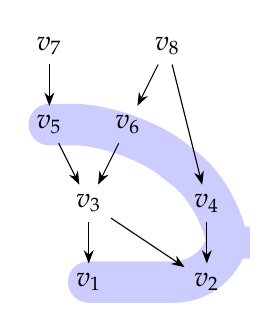
\begin{tikzpicture}
\begin{scope}[>={Stealth[black]},              
              every edge/.style={draw=black}]
    \node (A) at (0.5,0) {$v_1$};
    \node (B) at (2,0) {$v_2$};
    \node (C) at (0.5,1) {$v_3$};
    \node (D) at (2,1) {$v_4$};
    \node (E) at (0,2) {$v_5$};
    \node (F) at (1,2) {$v_6$};
    \node (G) at (0,3) {$v_7$};    
    \node (H) at (1.5,3) {$v_8$};   
    \path [->] (G) edge (E);
    \path [->] (H) edge (F);
    \path [->] (H) edge (D);
    \path [->] (E) edge (C);
    \path [->] (F) edge (C);
    \path [->] (C) edge (A);
    \path [->] (C) edge (B);
    \path [->] (D) edge (B);
\end{scope}
% Highlight the A_1 -> B_1 -> C_2 path. Use layers to draw
% behind everything.
\begin{pgfonlayer}{background}
	\draw[rounded corners=2em,line width=1.5em,blue!20,cap=round]
		(A.center) -- (B.east) -- (D.east) -- (F.center) -- (E.center);
\end{pgfonlayer}
\end{tikzpicture}
\caption{A DAG, in which the Markov blanket of $v_3$ is $\{v_5,v_6,v_1,v_2,v_4\}$.}
\label{fg:mb_example}
\end{figure}
Since 19xx, researchers have been developing efficient algorithms for learning Markov blankets from observational data (many citations). Due to the complexity of the problem, most of these learners are heuristics based on either statistical significant tests or objective functions for optimally balancing between predictive power and complexity. A set of subsets of variables $B=\{B_1, \dots, B_n\}$, one for each variable $v_i \in V$, which are learned from a Markov blanket learner must satisfy the symmetric and consistent properties for $B$ being a valid set of Markov blankets. The symmetric property is a direct consequence of the graphical interpretation of Markov blankets in a directed acyclic graph (DAG). That is, $v_i \in B_j$ if and only if $v_j \in B_i$. The consistent property entails that there exists at least one DAG $G=(V,E)$ s.t. the set of parents, children and spouses of node $v_i \in V$ equals $B_i$ for all $v_i$ in $G$. 

Outputs of Markov blanket learners are generally used without explicitly knowing the role of each member in $B_i$ relative to the target variable $v_i$. This does not stop the symmetric property to be checked (and possibly enforced), but makes it non-trivial for checking their consistency (with a DAG). Without being consistent, a set of learned Markov blankets could lead to inconsistent local structures within Markov blankets, which has to be resolved at some stage during the transition from local to global structure learning. In this paper, we drew a connection between Markov blankets' consistency and graph morality, and presented algorithms for checking morality for undirected graphs with various of maximum degrees. The contribution of this paper is threefold. First, we introduced the concepts of \textit{weak recursively simplicial} and \textit{perfect elimination kit} to help checking morality and prove important properties of moral graphs that will be studied in future investigation. Second, we developed polynomial time algorithms for checking morality for maximum degree $3$ and $4$ graphs. And we proved that checking morality for graphs with maximum degree $5$ and above is NP-complete. Third, all the algorithms for checking morality, including a backtracking algorithm for graphs with maximum degree $5$ and above, give a way of \textit{immoralizing} moral graphs to obtain DAGs. 


\section{Preliminary} 
In this section, we introduced the a few graph theory concepts that lead to Bayesian networks, moral graphs and chordal graphs. We then introduced several new concepts that are proved to be equivalent as graph morality in the next section, and consequently are used for proving the complexity in Section \ref{sec:complexity}. 

\begin{definition}
\label{def:graph}
A \textbf{graph} is a pair $G = (V, E)$ comprising a set $V$ of vertices (or nodes) together with a set $E$ of edges (or arcs).
\end{definition}

\begin{definition}
\label{def:digraph}
A \textbf{directed graph} is a graph $G=(V,E)$, where $E$ is a set of ordered pairs of distinct vertices in $V$.
\end{definition} 

\begin{definition}
\label{def:hybrid_g}
A \textbf{hybrid graph} is a graph consisting of both directed and undirected edges. 
\end{definition}
Later in this section, we introduced moral graphs, which require the direction of a directed edge to be dropped. Hence, if $G=(V,E)$ is a directed graph, we use $U(G)$ to denote the undirected version of $G$ and $U(E)$ to denote the undirected version of $G$'s edges. 

\begin{definition}
A \textbf{path} is a graph $P=(V,E)$, whose vertex set $V=\{v_1,v_2,\dots,v_{n-1},v_n\}$ and edge set $E=\{v_1v_2,\dots,v_{n-1}v_n\}$, where $v_i\neq v_j$ for $i,j \in [1,n]$.
\end{definition}
We use $P=v_1\dots v_k$ to denote a path between $v_1$ and $v_k$. The path $P$ has length $k$, denoted by $|P|=k$.

\begin{definition}
A \textbf{cycle} is a closed path $P=v_1\dots v_{k+1}$ where $v_i\neq v_j$ for $i,j \in [1,k]$ and $v_1=v_{k+1}$. 
\end{definition}
A cycle of length $m$ is called an m-cycle, denoted by $C_m$. 

\begin{definition}
A graph is \textbf{connected} if every pair of vertices are connected by a path. 
\end{definition}
The vertex and edge set of $G$ is denoted by $V(G)$ and $E(G)$ respectively. Throughout this paper, we use $u,v$ to represent vertices in $V$ and $uv$ to represent an (undirected) edge in $E$. A graph refers to a connected undirected graph, unless it is said otherwise. 

\begin{definition}
\label{def:dag}
A directed graph $G = (V, E)$ is called a \textbf{directed acyclic graph} if it contains no directed cycles. 
\end{definition}
In a directed acyclic graph $G=(V,E)$, $u$ is a \textit{parent} of $v$, denoted by $u \in P(v)$ (or $v$ is a \textit{child} of $u$), if there is a directed edge from $u$ to $v$. And $u$ is an \textit{ancestor} of $v$ (or $v$ is a \textit{descendent} of $u$) if there is a directed path from $u$ to $v$. Furthermore, $v$ is a \textit{nondescendent} of $u$ if $v$ is not a descendent of $u$.

\begin{definition}
\label{def:markov}
Let $\mathcal{P}$ be a joint probability distribution of the random variables in $V$, and $G=(V,E)$ be a directed acyclic graph. We say $<G, \mathcal{P}>$ satisfies the \textbf{Markov condition} if for every variable $v_i \in V$, it is conditionally independent of its non-descendants  given its parents set.
\end{definition}

\begin{definition}
\label{def:bn}
Let $\mathcal{P}$ be a joint probability distribution of the random variables in $V$, and $G=(V,E)$ be a directed acyclic graph. We say $<G, \mathcal{P}>$ forms a \textbf{Bayesian network} if it satisfies the Markov condition. 
\end{definition}

\begin{definition}
A Bayesian network $<G, \mathcal{P}>$ satisfies the \textbf{faithfulness} condition if the only conditional independencies in $\mathcal{P}$ are those entailed by the Markov condition. 
\end{definition}

\begin{definition}
\label{def:mb}
Let $<G=(V,E),\mathcal{P}>$ be a Bayesian network. The \textbf{Markov blanket} of $u$ in the Bayesian network, denoted by $B(u)$, is the minimum subset of variables s.t. $u \!\perp\!\!\!\perp_{\mathcal{P}} v \mid B(u)$ for each $v \in V\setminus B[u]$, where $B[u]=B(u)\cup \{u\}$.
\end{definition}

\iffalse
\begin{definition}
\label{def:skeleton}
The \textbf{skeleton} of a hybrid graph is the undirected graph obtained by dropping directions of all directed edges. 
\end{definition} 
\fi

\begin{definition}
\label{def:moral_g}
The \textbf{moral graph} of a directed acyclic graph $G=(V,E)$ is an undirected graph $H=(V,U(E) \cup F)$, where $F=\{uv \notin U(E) \mid u,v \in P_G(x),\forall x\in V\}$ is the set of filled edges. 
\end{definition}
The above definition implicitly states a way of obtaining a moral graph from a DAG. That is, by joining all pairs of non-adjacent parents in the DAG, then dropping all the directions. The process of obtaining a moral graph from a DAG is also known as \textit{moralization}. 

\begin{example}
Figure \ref{fg:envelope} shows a DAG $G$ and its moral graph $H$ that is obtained by joining $v_3$ and $v_4$ then dropping all the directions in the hybrid graph. 
\label{ex:moral_graph}
\begin{figure}[H]
\centering
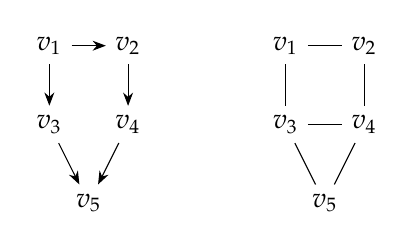
\begin{tikzpicture}
%\tikzstyle{place}=[circle,draw=blue!50,fill=blue!20,thick,inner sep=0pt,minimum size=6mm]
\begin{scope}
    \node (A) at (0,0) {$v_1$};
    \node (B) at (1,0) {$v_2$};
    \node (C) at (0,-1) {$v_3$};
    \node (D) at (1,-1) {$v_4$};
    \node (E) at (0.5,-2) {$v_5$};
    
    \node (F) at (3,0) {$v_1$};
    \node (G) at (4,0) {$v_2$};
    \node (H) at (3,-1) {$v_3$};
    \node (I) at (4,-1) {$v_4$};
    \node (J) at (3.5,-2) {$v_5$};
\end{scope}

\begin{scope}[>={Stealth[black]},
              every node/.style={fill=white,circle},
              every edge/.style={draw=black}]
    \path [->] (A) edge (B);
    \path [->] (A) edge (C);
    \path [->] (B) edge (D);
    \path [->] (C) edge (E);
    \path [->] (D) edge (E);
    
    \path [-] (F) edge (G);
    \path [-] (F) edge (H);
    \path [-] (G) edge (I);
    \path [-] (H) edge (I);
    \path [-] (H) edge (J);
    \path [-] (I) edge (J);
%    \path [-] (B) edge [bend right=60] (E); 
\end{scope}
\end{tikzpicture}
\caption{A DAG $G=(V,E)$ and its moral graph $H=(V,U(E)\cup F)$, in which $v_3v_4 \in F$ is a filled edge.}
\label{fg:envelope}
\end{figure}
\end{example}

If a given Bayesian network $<G=(V,E),\mathcal{P}>$ is faithful, the Markov blanket of a variable $u$ consists of its parents, children and children's other parents. For any spouse $v$ of $u$ that is neither a parent nor child of $u$, the edge $uv$ is a filled edge to make the moral graph $H$ of $G$. Hence, for each node $u \in V$, there is a one-to-one correspondence between its Markov blanket in $G$ and its neighbourhood in $H$. For example, in Figure \ref{fg:envelope} $B_G(v_3)=\{v_1,v_5,v_4\}=N_H(v_3)$.
\begin{definition}
\label{def:collider}
A \textbf{collider} in a hybrid graph is a node with at least two parents. 
\end{definition}

\begin{definition}
\label{def:consistent_ext}
A directed acyclic graph $G=(V,E)$ is a \textbf{consistent extension} of a hybrid graph $H=(V,F)$ if $U(E)=U(F)$ and $G$ and $H$ have the same set of colliders. 
\end{definition}

\begin{definition}
\label{def:subgraph}
Let $G'=(V',E')$ and $G=(V,E)$ be two graphs. If $V' \subseteq V$ and $E' \subseteq E$, then $G'$ is a \textbf{subgraph} of $G$, written as $G' \subseteq G$. 
\end{definition}

\begin{definition}
\label{def:induced_subgraph}
Let $G'=(V',E')$ and $G=(V,E)$ be two graphs. If $G'\subseteq G$ and $uv \in E$ for all $u,v \in V'$, then $G'$ is an \textbf{induced subgraph} of $G$, written as $G'=G[V']$.
\end{definition}
For simplicity, if $V' \subset V$ then we use $G-V'$ to denote $G[V\setminus V']$. If $V'=\{u\}$, then we use $G-u$. If $V'=V(H)$, then we use $G-H$. Similarly, if $E' \subset E$ then we use $G+E'$ and $G-E'$ to denote $(V,E \cup E')$  and $(V,E\setminus E')$ respectively. If $E' = \{uv\}$ then we use $G+uv$ or $G-uv$ instead.

\begin{definition}
Let $G=(V,E)$ be a graph. The set of \textbf{neighbours} of $u$ in $G$ is $N(u)=\{v \in V \mid uv \in E\}$. The closed neighbourhood of $u$ in $G$ is $N[u]=N(u)\cup \{u\}$.
\end{definition}
It is also useful to define the neighbours of a subgraph $H \subset G$ as $N_G(H)=\{u \in V\setminus V(H) \mid uv \in E, \forall v \in V(H)\}$.

\begin{definition}
Let $G=(V,E)$ be a graph. The \textbf{maximum degree} of the graph is $\Delta(G)=\max\{d(u) \mid u \in V\}$, where $d(u)=|N(u)|$ is the degree of $u$.
\end{definition}

\begin{definition}
A \textbf{clique} is a subset of nodes in a graph where every two distinct nodes are adjacent. 
\end{definition}

\begin{definition}
A \textbf{simplicial node} in a graph is a node whose neighbours form a clique. 
\end{definition}

\begin{definition}
Let $G=(V,E)$ be a graph. The \textbf{deficiency} of a node $x$ in $G$ is $D(x)=\{uv \notin E \mid u, v \in N(x)\}$.
\end{definition}
A node $u$ is simplicial in $G$ if and only if $D(u)=\emptyset$. That is, no edge needs to be filled in to make the neighbours of $u$ a clique. We write $D(G)\neq \emptyset$ if $D_G(u)\neq \emptyset, \forall u \in V$. And $D(G)=\emptyset$ if $\exists x \in V$ s.t. $D(x)=\emptyset$.
\begin{example}
In the moral graph $H$ as shown in Figure \ref{fg:envelope}, $D_H(v_1)=\{v_2v_3\}$ and $D_H(v_5)=\emptyset$. 
\end{example}

\begin{definition}
A \textbf{chord} in a m-cycle $C_m=v_1\dots v_mv_1$ is an edge $v_iv_j \notin E(C_m)$ for $i,j \in [1,m]$.
\end{definition}

\begin{definition}
A graph is \textbf{chordal} if each m-cycle for $m \ge 4$ has a chord.
\end{definition}

\begin{definition}
An \textbf{ordering} of a graph $G=(V,E)$ with $n$ vertices is a bijection $\alpha: \{1, \dots, n\} \leftrightarrow V$. 
\end{definition}
Another equivalent property as being chordal is that $G$ has a \textit{perfect elimination ordering}. That is, for each $x \in V$ with $\alpha^{-1}(x)=i+1$, we have $D_{G^i}(x)=\emptyset$, where $G^i=G-\{\alpha(1),\dots,\alpha(i)\}$ and $G^0=G$.

\begin{definition}
A graph $G=(V,E)$ is \textbf{recursively simplicial} if $\exists x \in V$ with $D_G(x)=\emptyset$ s.t. the induced subgraph $G-x$ is recursively simplicial. 
\end{definition}
Being recursively simplicial is equivalent as being chordal. It makes chordality a hereditary property. The following concept is not as strong as recursively simplicial, so it requires some edges to be removed in addition to the removal of a simplicial node. 

\begin{definition}
\label{def:wrs}
A graph $G=(V,E)$ is \textbf{weak recursively simplicial} if $\exists x \in V$ with $D_G(x)=\emptyset$ and $\exists E'\subseteq \{uv \in E \mid u,v \in N_G(x)\}$ s.t. the subgraph $G'=G-x-E'$ is weak recursively simplicial. 
\end{definition}

\begin{example}
\begin{figure}[H]
\centering
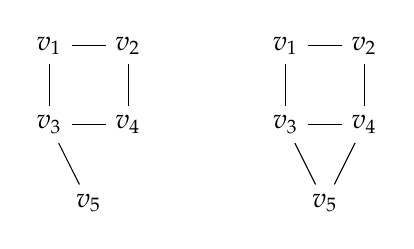
\begin{tikzpicture}
%\tikzstyle{place}=[circle,draw=blue!50,fill=blue!20,thick,inner sep=0pt,minimum size=6mm]
\begin{scope}
    \node (A) at (0,0) {$v_1$};
    \node (B) at (1,0) {$v_2$};
    \node (C) at (0,-1) {$v_3$};
    \node (D) at (1,-1) {$v_4$};
    \node (E) at (0.5,-2) {$v_5$};
    
    \node (F) at (3,0) {$v_1$};
    \node (G) at (4,0) {$v_2$};
    \node (H) at (3,-1) {$v_3$};
    \node (I) at (4,-1) {$v_4$};
    \node (J) at (3.5,-2) {$v_5$};
\end{scope}

\begin{scope}[>={Stealth[black]},
              every node/.style={fill=white,circle},
              every edge/.style={draw=black}]
    \path [-] (A) edge (B);
    \path [-] (A) edge (C);
    \path [-] (B) edge (D);
    \path [-] (C) edge (D);
    \path [-] (C) edge (E);
    
    \path [-] (F) edge (G);
    \path [-] (F) edge (H);
    \path [-] (G) edge (I);
    \path [-] (H) edge (I);
    \path [-] (H) edge (J);
    \path [-] (I) edge (J);
%    \path [-] (B) edge [bend right=60] (E); 
\end{scope}
\end{tikzpicture}
\caption{An example of a non-weak recursively simplicial graph $G$ (left) and a weak recursively simplicial graph $H$ (right).}
\label{fg:wrs}
\end{figure}

$H$ is a weak recursively simplicial (WRS) graph that can be justified by the following two criterion:
\begin{enumerate}
\item recursively removing $\{v_5, v_3v_4\}$, $\{v_3\}$, $\{v_4\}$, $\{v_1\}$, $\{v_2\}$ to eliminate the graph completely,
\item each node removed is a simplicial node in the current graph.
\end{enumerate}
On the other hand, the graph $G$ is not WRS, because there is no way $G$ can be eliminated completely whilst the node removed at each step is simplicial in the current graph. 
\end{example}

If a graph is recursively simplicial (i.e., chordal), it is also weak recursively simplicial with $E'=\emptyset$ for each simplicial node $x$. The converse, however, is not true. For example, the graph $H$ in Figure \ref{fg:wrs} is WRS but not chordal. 

\begin{definition}
A set of \textbf{excesses} of a graph $G=(V,E)$ according to an ordering $\alpha$ is a bijection $\epsilon_{\alpha}: \alpha \leftrightarrow \{\epsilon_{\alpha}(v_1), \dots, \epsilon_{\alpha}(v_n)\}$, where each $\epsilon_{\alpha}(v_i) \subseteq E(G[N(v_i)])$ consists of some edges between the neighbours of $v_i$.
\end{definition}
The composition $\kappa=(\alpha,\epsilon_{\alpha})$ of an ordering and a set of excesses is called an elimination kit of a graph $G$. We use $\kappa(1)$ to denote the node $\alpha(1)$ and its excess $\epsilon_{\alpha}(\alpha(1))$. By using the concept of elimination kit, we extend the definition of the subgraph $G^i=G-\{\kappa(1),\dots,\kappa(i)\} \subset G$ for $i\in [1,n]$, with the same convention $G^0=G$. 

\begin{example}
\label{ex:ek}
An ordering $\alpha=(v_5,v_3,v_4,v_1,v_2)$ and a set of excesses $\epsilon_{\alpha}=(\emptyset,\emptyset,\emptyset,\emptyset,\emptyset)$ form an elimination kit of $H$ in Figure \ref{fg:envelope}. 
\end{example}

\begin{definition}
Let $G=(V,E)$ be a graph and $\kappa=(\alpha, \epsilon_{\alpha})$ be an elimination kit of $G$. It is a \textbf{perfect elimination kit} if for each $x \in V$ with $\alpha^{-1}(x)=i+1$, we have $D_{G^{i}}(x)=\emptyset$.
\end{definition}
If a graph $G$ admits a perfect elimination kit (pek), there may exists $x \in V$ that is simplicial in a subgraph $G^i$, but not simplicial in $G$. We call such $x$ a \textit{local simplicial} node. In general, a graph may have none, one or more than one perfect elimination kit. 
\begin{example}
\label{ex:pek}
The elimination kit in Example \ref{ex:ek} is not perfect, because $D_{G^1}(v_3)\neq \emptyset$. The only pek for $H$ is $\alpha=(v_5,v_3,v_4,v_1,v_2)$ and $\epsilon_{\alpha}=(\{v_3v_4\},\emptyset,\emptyset,\emptyset,\emptyset)$. 
\end{example}

\begin{definition}
Let $G=(V,E)$ be a graph and $\kappa=(\alpha, \epsilon_{\alpha})$ be an elimination kit of $G$. It is a \textbf{partial perfect elimination kit} if there exists a non-empty subgraph $G^i \subset G$ s.t. $D(G^i)\neq \emptyset$ and $D_{G^{j-1}}(\alpha(j))=\emptyset$ for $j \in [1,i]$.
\end{definition}
A 4-cycle has no partial pek, because it has no simplicial node. A graph that has a pek may also has a partial pek.
\begin{example}
Example \ref{ex:ek} is a partial pek, because $D(G^1)\neq \emptyset$ and $D_{G^0}(v_5)=\emptyset$. 
\end{example}


\section{Weak recursively simplicial graphs}
The first main task of this section is to prove there is a one-to-one correspondence between moral graphs and weak recursively simplicial graphs. To do this, we prove the following two lemmas. 

\begin{lemma}
\label{lm:moral_implies_wrs}
Let $G=(V,E)$ be a DAG and $H$ be the moral graph of $G$. Then $H$ is weak recursively simplicial. 
\end{lemma}

\begin{proof}
The lemma is proved by induction on the number of nodes. Let $G(n)$ and $H(n)$ denote a DAG and its moral graph over a set of $n$ nodes. The lemma is true for $n \le 3$, because all graphs contain three nodes or less are WRS. Assuming $H(n)$ is WRS for an arbitrary $n \ge 4$. We want to show that the moral graph $H(n+1)$ is also WRS. It is known that each DAG contains at least one sink $x$, and $x$ becomes a simplicial node in the DAG's moral graph because its parents form a clique after moralization. Hence, the moral graph $H(n+1)$ contains a simplicial node $x$. By removing $x$ and the edges that were introduced by moralization to make $x$'s neighbours a clique, the resulting graph $H(n)$ is the moral graph of the DAG $G(n)$ obtained by removing $x$ from $G(n+1)$. The inductive hypothesis assumes that each moral graph $H(n)$ is WRS. Hence, $H(n+1)$ is also WRS. \qed
\end{proof}
Lemma \ref{lm:moral_implies_wrs} suggests that the moral graph of any DAG is WRS. To prove there is a one-to-one correspondence it is remaining to show that the converse is also true. That is, a WRS graph is the moral graph of a DAG. 

\begin{lemma}
\label{lm:wrs_implies_moral}
Let $H=(V,E)$ be a weak recursively simplicial graph. Then $H$ is the moral graph of a DAG. 
\end{lemma}

\begin{proof}
The lemma is proved by induction on the number of nodes $n$. The statement is true for $n=1$, because a single node graph $H(1)$ is both the moral graph of $G(1)$ and a WRS graph. Assuming the lemma is true for an arbitrary $n\ge 2$. That is, any WRS graph $H(n)$ with $n\ge 2$ is the moral graph of a DAG $G(n)$. Each WRS graph has a simplicial node. Assuming $x$ is a simplicial node of a WRS graph $H(n+1)$ and $x$ is the first in the ordering $\alpha$ (i.e., $\alpha^{-1}(x)=1$). When orienting $H(n+1)$, we first let all the edges connect to $x$ be directed towards it. Furthermore, some edges between the neighbours of $x$ are removed so that the resulting graph $H(n)$ is still WRS. By the inductive assumption, $H(n)$ is the moral graph of a $G(n)$. Hence, by attaching $x$ and the edges connect to it onto $G(n)$ we obtain a DAG $G(n+1)$, whose moral graph is $H(n+1)$. \qed
\end{proof}

\begin{theorem}
\label{thm:wrs_equal_moral}
A graph is weak recursively simplicial if and only if it is the moral graph of a DAG. 
\end{theorem}
\begin{proof}
The theorem follows from Lemma \ref{lm:moral_implies_wrs} and Lemma \ref{lm:wrs_implies_moral}. \qed
\end{proof}
Moralization from a DAG to an undirected graph is trivial, whilst orienting a moral graph to obtain a DAG with the same Markov blankets is not trivial. It is beyond the focus of this paper but is an interesting topic that worth further investigating. It has a potential to unify a (symmetric and consistent) set of Markov blankets to obtain a DAG, which may not be the generating model, but could be used as a start for heuristic structure learning and causal discovery algorithms. 

Chordality is considered to be a \textit{hereditary} property of a graph, because the subgraph is still chordal after removing a simplicial node from a chordal graph. Similarly, morality is also a hereditary property, but in the sense that the subgraph is still moral after removing a simplicial node and some edges between its neighbours from a moral graph. 

\iffalse
% this result is not difficult, but doesn't fit the content of this paper. 
\begin{corollary}
Let $\mathcal{F}=\{F=(V,E) \mid F \text{ is weak recursively simplicial}\}$ be the set of weak recursively simplicial graphs over $V$ and $\mathcal{B} = \{B_V^G \mid \text{for all DAG $G$ over $V$}\}$ be the set of Markov blanket families of any DAG over $V$. Then $|\mathcal{F}| = |\mathcal{B}|$. 
\end{corollary}
\begin{proof}
It is straightforward that there is a one-to-one correspondence between $\mathcal{B}$ and moral graphs. Hence, Corollary \ref{cor:wrs_equal_moral} implies that $\mathcal{F}$ has a one-to-one correspondence with $\mathcal{B}$, so equal cardinality. \qed
\end{proof}
\fi

Next, we present a backtracking algorithm for checking whether or not a given graph $G=(V,E)$ is WRS. If it is, the algorithm will return TRUE and orient it into a hybrid graph that always has a consistent DAG extension \cite{dor1992simple}, whose Markov blankets are identical to $G$'s.
\begin{algorithm}[]
\caption{Checking morality using backtracking}
\label{alg:wrs_bktr}
\begin{algorithmic}[]
	\Require{a graph $G=(V,E)$}
	
    \Function{$\phi$}{$F$}
    \If{$G=\emptyset$}     
    	\Return {TRUE} 
    \EndIf
    
    \If{$D(G)=\emptyset$}
    	\State $H = G$ \Comment{cache $G$}
    	\ForEach{$x \in V(G)$ s.t. $D_G(x)=\emptyset$} \Comment{for each simplicial node}
    		\State $E'=\{uv \in E(G) \mid u,v\in N_G(x)\}$
    		\ForEach{$\epsilon(x) \subseteq E'$} \Comment{for each excess}
    			\State $G=H$ \Comment{restore $G$}
    			\State $G=G-x-\epsilon(x)$ 
        		\If{$\phi(F)=$ TRUE}         		
        			\Return {TRUE} \Comment{apply recursion}
        		\EndIf
      		\EndFor
      	\EndFor
    \EndIf
    
    \State \Return{FALSE} \Comment{return FALSE if no simplicial node}
    \EndFunction
\end{algorithmic}
\end{algorithm}

So far, we have proved a one-to-one correspondence between moral graphs and WRS graphs. The following theorem proves that being WRS is the same as having a pek.  

\begin{theorem}
A graph is weak recursively simplicial if and only if has a perfect elimination kit. 
\end{theorem}
\begin{proof}
If $G=(V,E)$ is WRS, the simplicial node $x$ and the edges $E' \subset E(G[N_G(x)])$ removed at each step of the recursion form an ordering and a set of excesses, because the $x$ at each step of the recursion is local simplicial. Hence, $G$ admits a pek. The converse is also true because if $G$ admits a pek, it can be eliminated recursively to the empty graph.\qed
\end{proof}

\iffalse
\begin{definition}
Given a cycle, an \textbf{n-chord} is defined as a path of length $n$ connecting two points on the cycle, where $n$ is less than the shortest path on the cycle connecting those points. 
\end{definition}

\begin{definition}
An \textbf{atomic cycle} is a cycle with no n-chord. 
\end{definition}
\fi

\citeauthor{verma1993deciding} \shortcite{verma1993deciding} made the following two remarks that could increase the speed of checking morality. 
\begin{remark}
If a graph is moral, it has at least one simplicial node. 
\end{remark}

\begin{remark}
If a graph is moral, each cycle in it shares an edge with a k-clique. 
\end{remark} 


\section{Complexity}
To check whether a graph $G$ is WRS (or has a pek), it involves removing a subset of edges between the neighbours of a simplicial node. Not only because the number of subsets increases exponentially in the degree of a simplicial node, but a selection of subset could affect future options, which can not be anticipated at the time of selection, the problem of checking morality is difficult in general. \citeauthor{verma1993deciding}\shortcite{verma1993deciding} proved that this problem is NP-complete for arbitrary graphs. In this section, we proved that for graphs with maximum degree less than $5$, their morality can be checked in polynomial time. We presented algorithms for graphs with maximum degree $3$ and $4$. Furthermore, we revised the proof by \citeauthor{verma1993deciding} so that the NP-completeness argument holds true for graphs with maximum degree $5$. 

If a graph is not connected, the morality of every connected component of it will be checked separately. Without loss of generality, we assume all graphs are connected. If a graph $G$ has $\Delta(G)=0$, it is a single node. If $\Delta(G)=1$, it is an single edge. If $\Delta(G)=2$, it is either a path or a simple cycle. Therefore, the morality of a graph $G$ with $\Delta(G)\le 2$ can be checked efficiently. To prove a polynomial time algorithm for checking maximum degree $3$ graphs, we prove the following lemmas first. 

\begin{lemma}
\label{lm:no_common_nbr}
If $G=(V,E)$ is not moral, then $H=G+uv$ is not moral for any pair of non-adjacent $u,v$ s.t. $N_G(u)\cap N_G(v)=\emptyset$. 
\end{lemma}
\begin{proof}
$G$ is not moral implies the following two cases:

\textit{Case 1:} $D(G)\neq \emptyset$. The only possibility for turning a node $x$ to simplicial in $H$ is when $D_G(x)=uv$. This contradicts with the premise $N_G(u)\cap N_G(v)=\emptyset$. Hence, $D(H)\neq \emptyset$.

\textit{Case 2:} $D(G)=\emptyset$. Then $G$ has only partial peks, each of which gives a subgraph $G^i \subset G$ s.t. $D(G^i)\neq \emptyset$. To make a node $x \in V(G^i)$ simplicial, either $D_{G^i}(x)=uv$ or $u \notin V(G^i)$ is a local simplicial node s.t. $|N_G(u) \cap V(G^i)| = 1$ and $v \in V(G^i)$ forms a clique with $N_G(u)$. Both conditions, however, contradict with $N_G(u)\cap N_G(v)=\emptyset$. Hence, $D(H)\neq \emptyset$. \qed
\end{proof}

\begin{lemma}
\label{lm:1kp}
Let $G=(V,E)$ be a moral graph. If $\exists x \in V$ with $D_G(x)=\emptyset$ s.t. for each pair $u, v \in N_G(x)$, their common neighbours $N_G(u)\cap N_G(v) \subset N_G[x]$, then $G'=G-x-E(G[N_G(x)])$ is moral.
\end{lemma}
\begin{proof}
Assume $G'$ is not moral. The removal of $E(G[N_G(x)])$ implies every pair of neighbours $u,v \in N_G(x)$ are non-adjacent in $G'$. In addition, $N_G(u)\cap N_G(v) \subset N_G[x]$ implies $N_{G'}(u)\cap N_{G'}(v)=\emptyset$. By Lemma \ref{lm:no_common_nbr}, the subgraph $G''=G-x-S$ is not moral for any proper subset $S \subsetneq E(G[N_G[x]])$. Without loss of generality, assuming $\alpha^{-1}(x)=1$, so $\nexists \epsilon_{\alpha}(x) \subset E(G[N_G(x)])$ s.t. the subgraph $G-x-\epsilon_{\alpha}(x)$ is moral. This contradicts with $G$ being moral. \qed
\end{proof}
\begin{lemma}
\label{lm:wrs_deg3}
Let $G=(V,E)$ be a moral graph with maximum degree $\Delta(G)=3$. If $\exists x \in V$ with $D_G(x)=\emptyset$, then $G'=G-x-E(G[N_G(x)])$ is moral. 
\end{lemma}
\begin{proof}
When $d_G(x)=3$, the graph $G=K_4$ so $G'$ is moral. When $d_G(x)=1$, $x$ is a leaf. Hence, $E(G[N_G(x)])=\emptyset$ and consequently $G'$ is moral.
\begin{figure}[H]
\centering
\begin{tikzpicture}
%\tikzstyle{place}=[circle,draw=blue!50,fill=blue!20,thick,inner sep=0pt,minimum size=6mm]
\begin{scope}           
    \node (a) at (0,0.5) {$x$};
    \node (b) at (1,0) {$u$};
    \node (c) at (1,1) {$v$};  
        
    \path [-] (a) edge (c);
    \path [-] (a) edge (b);
    \path [-] (c) edge (b);
\end{scope}
\draw[dashed] (b) .. controls (3,0) and (3,1) .. (c);
\end{tikzpicture}
\caption{A graph $G$ with $\Delta(G)=3$ and $D_G(x)=\emptyset$.}
\label{fg:deg3_1k3}
\end{figure}
For the case when $d_G(x)=2$, assume $N_G(x)=\{u,v\}$ (Figure \ref{fg:deg3_1k3}). If the edge $uv$ is not in a cycle in $G-x$, then $G'$ is moral. Suppose $uv \in E(C_m)$ is in a m-cycle. If $m=3$, then $\exists w \neq x$ s.t. $w \in N_G(u) \cap N_G(v)$. It entails the induced subgraph $H=G[\{x,u,v,w\}])$ is triangulated. $d_G(u)=d_G(v)=\Delta(G)$ and $d_G(w)=2$ suggest $N_G(H)=y \in V(G-H)$ and $wy \in E$. That is, the rest of the graph is connected to $H$ via a single edge $wy$ only. Hence, $G'$ is moral. If $m\ge 4$, the graph $G$ satisfies the conditions in Lemma \ref{lm:1kp}, hence $G'$ is moral. \qed
\end{proof}

\begin{algorithm}[]
\caption{Checking morality for maximum degree 3 graphs}
\label{alg:wrs_deg3}
\begin{algorithmic}[]
	\Require{a graph $G=(V,E)$ with $\Delta(G)=3$}   
    
    \While{$\exists x$ s.t. $D_G(x)=\emptyset$}    	
    	\State $G=G-x-E(G[N_G(x)])$    	
    \EndWhile
       
    \If{$G=\emptyset$}    
     
    	\Return {TRUE} 
    \Else 
    
    	\Return{FALSE}
    \EndIf
\end{algorithmic}
\end{algorithm}

\begin{theorem}
\label{thm:wrs_deg3}
The morality of maximum degree $3$ graphs can be check in polynomial time. 
\end{theorem}
\begin{proof}
A straightforward algorithm (Algorithm \ref{alg:wrs_deg3}) for checking morality for maximum degree $3$ graphs can be deduced directly from Lemma \ref{lm:wrs_deg3}. If $G$ is moral, Algorithm \ref{alg:wrs_deg3} stops till $G$ is empty and returns TRUE, else it stops at a non-empty subgraph of $G$ and returns FALSE. 

A graph $G$ with $|V|=n$ nodes can be represented by an adjacency list, from which it takes constant time to find $N(x)$ for $x \in V$. Since $|N(x)| \le \Delta(G)=3$, it takes constant time to verify $D(x)=\emptyset$. In the worst case scenario, the only simplicial node is always at the end of the list, so it takes $O(n)$ time to find it. The operations of removing $x$, $\{xy \in E\mid \forall y \in N_G(x)\}$ and $E(G[N(x)])$ take constant time. The while loop repeats at most $n$ times, so Algorithm \ref{alg:wrs_deg3} has computational complexity $O(n^2)$ and consequently is a polynomial time algorithm . \qed
\end{proof}
The complexity of Algorithm \ref{alg:wrs_deg3} may be reduced further by using a different data structure, but it is beyond the focus of this paper. \citeauthor{rose1976algorithmic} \shortcite{rose1976algorithmic} proved chordality can be checked in polynomial time using a specially-designed data structure. For graphs with maximum degree $4$, there are more cases to be considered. 

\begin{lemma}
\label{lm:deg1_4_3}
Let $G=(V,E)$ be a moral graph with $\Delta(G)=4$. If $\exists x \in V$ with $d_G(x)\in \{1,4,3\}$ and $D_G(x)=\emptyset$, then $G'=G-x-E(G[N(x)])$ is moral. 
\end{lemma}
\begin{proof}
For $x \in V$ with $D_G(x)=\emptyset$, if $d_G(x)=1$ then $x$ is a leaf, so $G'$ is moral. If $d_G(x)=4$, then $G=K_5$ is a complete graph so $G'$ is moral. If $d_G(x)=3$, the case is similar as $d_G(x)=2$ for a graph $G$ with maximum degree $\Delta(G)=3$ in the proof of Lemma \ref{lm:wrs_deg3}. Hence, $G'$ is moral. \qed
\end{proof}

\begin{lemma}
\label{lm:1k3}
Let $G=(V,E)$ be a moral graph with maximum degree $\Delta(G)=4$. If $\exists x \in V$ with $D_G(x)=\emptyset$ s.t. $N_G(x)=\{u,v\}$ and $N_G(u)\cap N_G(v)=\{x\}$, then $G'=G-x-E(G[N(x)])$ is moral.
\end{lemma}
\begin{proof}
It follows from Lemma \ref{lm:1kp}. \qed
\end{proof}
The above lemma states that if $x$ is a simplicial node that is in a $K_3$, then removing $x$ and the edges between each pair of its neighbours results in a moral subgraph. Let $K_3^m$ denote a stack of more than one $K_3$s. For example, Figure \ref{fg:2k3s} contains a $K_3^2$. The following lemmas prove the appropriate operations to obtain a moral subgraph from $G$ under different scenarios. 

\begin{lemma}
\label{lm:2k3s}
Let $G=(V,E)$ be a moral graph with maximum degree $\Delta(G)=4$. If $K_3^2 \subset G$ s.t. $\exists x\in V(K_3^2)$ with $d_G(x)=2$ and $D_G(x)=\emptyset$, then $G'=G-x$ is moral.
\begin{figure}[H]
\centering
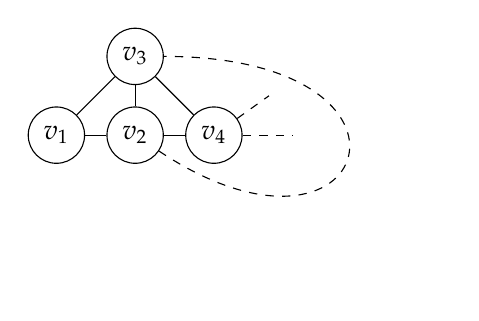
\begin{tikzpicture}
%\tikzstyle{place}=[circle,draw=blue!50,fill=blue!20,thick,inner sep=0pt,minimum size=6mm]
\begin{scope}[every node/.style={circle,draw}]               
    \node (a) at (0,0) {$v_1$};
    \node (b) at (1,0) {$v_2$};
    \node (c) at (1,1) {$v_3$};  
    \node (d) at (2,0) {$v_4$};
        
    \path [-] (a) edge (c);
    \path [-] (a) edge (b);
    \path [-] (b) edge (d);
    \path [-] (c) edge (b);
    \path [-] (c) edge (d);
    %\draw[dashed] (b) -- (2,-0.5);
    \draw[dashed] (d) -- (2.7,0.5);
    \draw[dashed] (d) -- (3,0);        
\end{scope}
\draw[dashed] (b) .. controls (4,-2) and (5,1) .. (c);
\end{tikzpicture}
\caption{A graph $G$ with $\Delta(G)=4$ and $K_3^2\subset G$.}
\label{fg:2k3s}
\end{figure}
\end{lemma}
\begin{proof}
Without loss of generality, assuming $K_3^3 \nsubset G$ and $G$ is labelled as shown in Figure \ref{fg:2k3s} with $v_1$ being simplicial. If $\exists u \in N_G(v_2)\cap N_G(v_3)$ s.t. $u \notin \{v_1,v_4\}$, then $H=G[\{v_1,v_2,v_3,v_4,u\}]\subset G$ is triangulated. $d_G(v_2)=d_G(v_3)=\Delta(G)$ implies $N_G(G-H)=\{v_4\}$. Hence, if $G$ is moral then $G'$ is moral. If there exists no such a node $u$, assuming $G'$ is not moral. To reach a contradiction with $G$ being moral, it is sufficient to show the subgraph $G''=G-x-v_2v_3$ is not moral. 

If the removal of the edge $v_2v_3$ renders more local simplicial nodes, then it must first turn either $v_2$ or $v_3$ into local simplicial in $G''$, provided neither of these two is local simplicial in $G'$. If neither $v_2$ nor $v_3$ is local simplicial in $G'$, then $d_{G'}(v_2)=d_{G'}(v_3)=3$ and $v_4$ is not local simplicial in $G'$. This implies $D_{G''}(v_2)\neq \emptyset$ and $D_{G''}(v_3) \neq \emptyset$. In addition, the assumption $K_3^3 \nsubset G$ entails $N_{G''}(v_2) \cap N_{G''}(v_4) = N_{G''}(v_3) \cap N_{G''}(v_4) = \emptyset$, so none of $v_2,v_3$ and $v_4$ is local simplicial in $G''$. Hence, $G''$ has no more local simplicial nodes than $G'$. Furthermore, since $E(G'') \subsetneq E(G')$, the set of all partial peks of $G''$ is a proper subset of the set of all partial peks of $G'$. Therefore, $G''$ is not moral. \qed
\end{proof}

\begin{figure}[H]
\centering
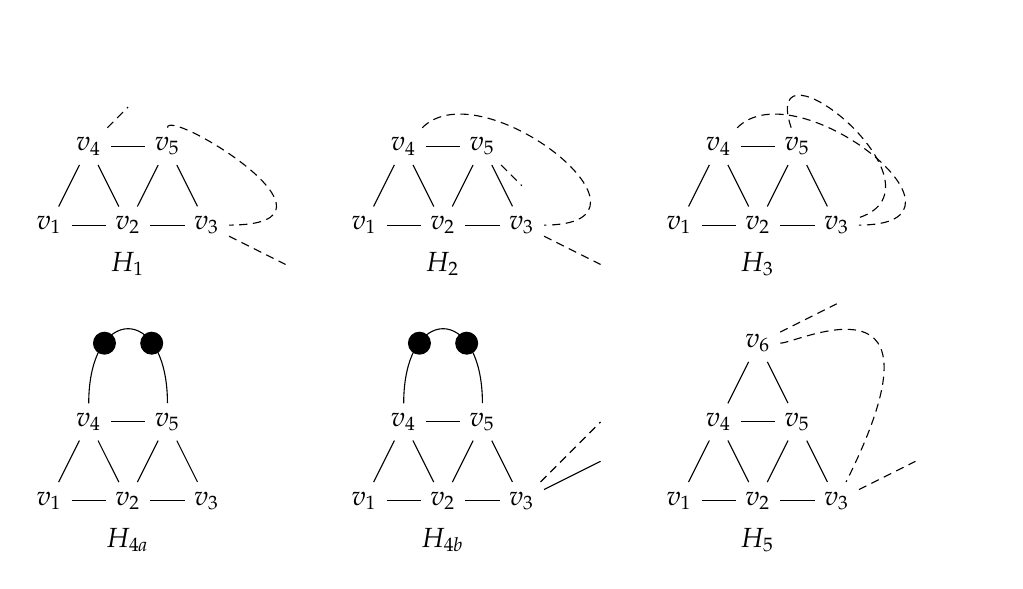
\begin{tikzpicture}
%\tikzstyle{place}=[circle,draw=blue!50,fill=blue!20,thick,inner sep=0pt,minimum size=6mm]
\begin{scope}              
    \node (A) at (-0.5,-2) {$v_1$};
    \node (B) at (1.5,-2) {$v_3$};
    \node (H) at (0,-1) {$v_4$};
    \node (I) at (1,-1) {$v_5$};
    \node (J) at (0.5,-2) {$v_2$};               
    \path [-] (A) edge (J);
    \path [-] (A) edge (H);
    \path [-] (B) edge (I);
    \path [-] (B) edge (J);
    \path [-] (H) edge (I);
    \path [-] (H) edge (J);
    \path [-] (I) edge (J); 
    \path [densely dashed] (H) edge (0.5,-0.5);
    \path [densely dashed] (B) edge (2.5,-2.5);
    
\end{scope}
\draw[densely dashed] (I) .. controls (1,-0.5) and (3.5,-2) .. (B);
\node at (0.5,-2.5) {$H_1$};

\begin{scope}              
    \node (A) at (3.5,-2) {$v_1$};
    \node (B) at (5.5,-2) {$v_3$};
    \node (H) at (4,-1) {$v_4$};
    \node (I) at (5,-1) {$v_5$};
    \node (J) at (4.5,-2) {$v_2$};               
    \path [-] (A) edge (J);
    \path [-] (A) edge (H);
    \path [-] (B) edge (I);
    \path [-] (B) edge (J);
    \path [-] (H) edge (I);
    \path [-] (H) edge (J);
    \path [-] (I) edge (J); 
    \path [densely dashed] (B) edge (6.5,-2.5); 
    \path [densely dashed] (I) edge (5.5,-1.5);       
\end{scope}
\draw[densely dashed] (H) .. controls (5,0) and (7.5,-2) .. (B);
\node at (4.5,-2.5) {$H_2$};

\begin{scope}              
    \node (A) at (3.5+4,-2) {$v_1$};
    \node (B) at (5.5+4,-2) {$v_3$};
    \node (H) at (4+4,-1) {$v_4$};
    \node (I) at (5+4,-1) {$v_5$};
    \node (J) at (4.5+4,-2) {$v_2$};               
    \path [-] (A) edge (J);
    \path [-] (A) edge (H);
    \path [-] (B) edge (I);
    \path [-] (B) edge (J);
    \path [-] (H) edge (I);
    \path [-] (H) edge (J);
    \path [-] (I) edge (J); 
    %\path [densely dashed] (B) edge (6.5+4,-2.5); 
    %\path [densely dashed] (I) edge (5.5+4,-1.5);       
\end{scope}
\draw[densely dashed] (I) .. controls (5+3.5,0.5) and (7.5+3.5,-1.5) .. (B);
\draw[densely dashed] (H) .. controls (5+4,0) and (7.5+4,-2) .. (B);
\node at (4.5+4,-2.5) {$H_{3}$};

\begin{scope}
    \node (a) at (3.5-4,-5.5) {$v_1$};
    \node (b) at (5.5-4,-5.5) {$v_3$};
    \node (h) at (4-4,-4.5) {$v_4$};
    \node (i) at (5-4,-4.5) {$v_5$};
    \node (j) at (4.5-4,-5.5) {$v_2$};           
    \path [-] (a) edge (j);
    \path [-] (a) edge (h);
    \path [-] (b) edge (i);
    \path [-] (b) edge (j);
    \path [-] (h) edge (i);
    \path [-] (h) edge (j);
    \path [-] (i) edge (j);
    \draw[-] (h) .. controls (0,-3) and (1,-3) .. (i);
    \foreach \Point in {(0.2,-3.5), (0.8,-3.5)}{
    \node[circle,draw,fill=black,minimum size=0.5mm,inner sep=0.3pt] at \Point {\textbullet};}
\end{scope}


\node at (0.5,-6) {$H_{4a}$};

\begin{scope}
    \node (a) at (3.5,-2-3-0.5) {$v_1$};
    \node (b) at (5.5,-5-0.5) {$v_3$};
    \node (h) at (4,-1-3-0.5) {$v_4$};
    \node (i) at (5,-1-3-0.5) {$v_5$};
    \node (j) at (4.5,-2-3-0.5) {$v_2$};           
    \path [-] (a) edge (j);
    \path [-] (a) edge (h);
    \path [-] (b) edge (i);
    \path [-] (b) edge (j);
    \path [-] (h) edge (i);
    \path [-] (h) edge (j);
    \path [-] (i) edge (j);
    \path [-] (b) edge (6.5,-4.5-0.5);
    \path [densely dashed] (b) edge (6.5,-4-0.5);  
    \foreach \Point in {(4.2,-3.5), (4.8,-3.5)}{
    \node[circle,draw,fill=black,minimum size=0.5mm,inner sep=0.3pt] at \Point {\textbullet};}  
\end{scope}
\draw[-] (h) .. controls (4,-2.5-0.5) and (5,-2.5-0.5) .. (i);
\node at (4.5,-5.5-0.5) {$H_{4b}$};

\begin{scope}
	\node (A) at (-0.5+8,-2-3-0.5) {$v_1$};
    \node (B) at (1.5+8,-2-3-0.5) {$v_3$};
    \node (F) at (0.5+8,0-3-0.5) {$v_6$};
    \node (H) at (0+8,-1-3-0.5) {$v_4$};
    \node (I) at (1+8,-1-3-0.5) {$v_5$};
    \node (J) at (0.5+8,-2-3-0.5) {$v_2$};  
	\path [-] (A) edge (J);
    \path [-] (A) edge (H);
    \path [-] (B) edge (I);
    \path [-] (B) edge (J);
    \path [-] (F) edge (H);
    \path [-] (F) edge (I);
    \path [-] (H) edge (I);
    \path [-] (H) edge (J);
    \path [-] (I) edge (J);
    \path [densely dashed] (F) edge (9.5,-2.5-0.5);
    \path [densely dashed] (B) edge (10.5,-4.5-0.5);    
\end{scope}
\draw[densely dashed] (F) .. controls (9,-3-0.5) and (11,-2-0.5) .. (B);
\node at (8.5,-5.5-0.5) {$H_5$};
\end{tikzpicture}
\caption{A list of all possible graphs $G$ with $\Delta(G)=4$ and $K_3^3\subset G$. Each dotted edge connects a node to a subgraph (possibly empty) of $G$. $H_5$ is a special case of $H_4$ when $N_{G}(v_4)\cap N_{G}(v_5)=\{v_2,v_6\}$.}
\label{fg:3k3s}
\end{figure}

\begin{lemma}
\label{lm:3k3s_h124}
Let $G=(V,E)$ be a moral graph with maxim degree $\Delta(G)=4$. If $K_3^3\subset G$ as shown in Figure \ref{fg:3k3s} s.t. $D_G(v_1)=\emptyset$ and $\min\{|P|\mid P=v_4\dots v_5 \subset G[V-\{v_1,v_2,v_3\}]-v_4v_5\} \in \{2, \infty\}$ , then $G'=G-v_1-E(G[N_G(v_1)])$ is moral.  
\end{lemma}
\begin{proof}
The premises of the lemma assume $G$ takes the form of either $H_1, H_2, H_3$ or $H_5$. We prove the lemma by contradiction. Assuming $G'$ is not moral, we want to reach a contradiction with the premise that $G$ is moral. To do so, we want to show that $G''$ is not moral either for $G''=G'+v_2v_4$. Clearly, $v_2$ is a simplicial node in $G'$. This implies $G'$ has only partial peks, each of which has a subgraph $G^i \subset G'$ s.t. $D(G^i)\neq \emptyset$. The addition of the edge $v_2v_4$ may turn a partial pek into a pek by rendering more local simplicial nodes or making use of existing local simplicial nodes, which could then be used to break cycles in $G^i$. Either case requires at least one of $v_2$ and $v_4$ to be in a m-cycle for $m \ge 4$ s.t. the cycle cannot be eliminated by any other clique in $G'$. None of the four graphs, however, satisfies the condition. Hence, $G''$ is not moral. \qed
\end{proof}

\begin{algorithm}[]
\caption{Checking morality for maximum degree $4$ graphs}
\label{alg:d_wrs_deg4}
\begin{algorithmic}[]
	\Require{a graph $G=(V,E)$ with $\Delta(G)=4$}
    
    \If{$\exists x$ s.t. $D_G(x)=\emptyset,d_G(x)=4$}
       \State \Return{TRUE}
    \EndIf
    
    \While {$D(G)=\emptyset$} \Comment{when $G$ has a simplicial node}
    
    \If{$\exists x$ s.t. $D_G(x)=\emptyset, d_G(x)=1$}
       \State $G=G-x$
    \ElsIf{$\exists x$ s.t. $D_G(x)=\emptyset,d_G(x)=3$}
       \State $G=G-x-E(G[N_G(x)])$
    \ElsIf{$\exists x \in K_3^m$ s.t. $D_G(x)=\emptyset$ for $m \ge 4$} \Comment{reduce long stack}
       \State $G=G-x-E(G[N_G(x)])$
    \ElsIf{$\exists x \in K_3$ s.t. $D_G(x)=\emptyset$}
       \State $G=G-x-E(G[N_G(x)])$
    \ElsIf{$\exists x \in K_3^2$ s.t. $D_G(x)=\emptyset$}
       \State $G=G-x$
    \Else \Comment{all simplicial nodes are in $K_3^3$}
    	\If{$\min\{|P|\mid P=v_4\dots v_5 \subset G-\{v_1,v_2,v_3\}-v_4v_5\} \in \{2, \infty\}$} \Comment{$H_1,H_2,H_3,H_5 \in G$}
    		\State $G=G-x-E(G[N_G(x)])$
    	\Else 
    		\If{$\exists y \in K_3^3$ s.t. $D_G(y)=\emptyset$ and $|N_G(x)\cap N_G(y)|=1$} \Comment{$H_{4a}\in G$}
       			\State $G=G-\{x,y\}$
   			\Else \Comment{$H_{4b} \in G$}
       			\State $G=G-x-E(G[N_G(x)])$
       		\EndIf
    	\EndIf
    	
       
    \EndIf
    
    \EndWhile
    
    \State \Return{FALSE}
    
\end{algorithmic}
\end{algorithm}

Algorithm \ref{alg:d_wrs_deg4} presents an efficient way of checking morality for graphs with maximum degree $4$. Its correctness and complexity are proved in Theorem \ref{thm:deg4}. The algorithm gets rid of simplicial nodes with degree $4,1$ and $3$ first. Then it deals with simplicial nodes with degree $2$, whose neighbours can adjacent to at most two other nodes. Within degree $2$ simplicial nodes cases, it identifies a long stack of $K_3$s (if there is any) and reduces its length recursively. Each time a simplicial node and the edge between its neighbours are removed, the length of the stack decreases by $2$ and eventually reaches $1,2$ or $3$, depending on the length of the original stack. It is worth mentioning that if $x \in K_3^3$, the cases have to be dealt in a fixed order. Counter examples are shown in Figure \ref{fg:fixed_order_example}, if the fixed order is not obeyed. 

\begin{figure}[H]
\centering
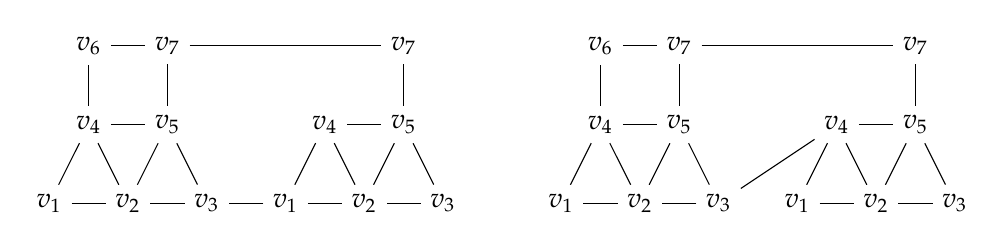
\begin{tikzpicture}
%\tikzstyle{place}=[circle,draw=blue!50,fill=blue!20,thick,inner sep=0pt,minimum size=6mm]
\begin{scope}              
    \node (A) at (-0.5,-2) {$v_1$};
    \node (B) at (1.5,-2) {$v_3$};
    \node (H) at (0,-1) {$v_4$};
    \node (I) at (1,-1) {$v_5$};
    \node (J) at (0.5,-2) {$v_2$};  
    \node (C) at (0,0) {$v_6$};
    \node (D) at (1,0) {$v_7$};    
    \path [-] (A) edge (J);
    \path [-] (A) edge (H);
    \path [-] (B) edge (I);
    \path [-] (B) edge (J);
    \path [-] (H) edge (I);
    \path [-] (H) edge (J);
    \path [-] (I) edge (J); 
    \path [-] (H) edge (C);
    \path [-] (C) edge (D);
    \path [-] (I) edge (D);
    
    \node (a) at (-0.5+3,-2) {$v_1$};
    \node (b) at (1.5+3,-2) {$v_3$};
    \node (h) at (0+3,-1) {$v_4$};
    \node (i) at (1+3,-1) {$v_5$};
    \node (j) at (0.5+3,-2) {$v_2$};
    \node (d) at (1+3,0) {$v_7$};
    \path [-] (a) edge (j);
    \path [-] (a) edge (h);
    \path [-] (b) edge (i);
    \path [-] (b) edge (j);
    \path [-] (h) edge (i);
    \path [-] (h) edge (j);
    \path [-] (i) edge (j);
    
    \path [-] (a) edge (B);
    \path [-] (D) edge (d);
    \path [-] (d) edge (i);
\end{scope}

\begin{scope}              
    \node (A) at (-0.5+6.5,-2) {$v_1$};
    \node (B) at (1.5+6.5,-2) {$v_3$};
    \node (H) at (0+6.5,-1) {$v_4$};
    \node (I) at (1+6.5,-1) {$v_5$};
    \node (J) at (0.5+6.5,-2) {$v_2$};  
    \node (C) at (0+6.5,0) {$v_6$};
    \node (D) at (1+6.5,0) {$v_7$};    
    \path [-] (A) edge (J);
    \path [-] (A) edge (H);
    \path [-] (B) edge (I);
    \path [-] (B) edge (J);
    \path [-] (H) edge (I);
    \path [-] (H) edge (J);
    \path [-] (I) edge (J); 
    \path [-] (H) edge (C);
    \path [-] (C) edge (D);
    \path [-] (I) edge (D);
    
    \node (a) at (-0.5+3+6.5,-2) {$v_1$};
    \node (b) at (1.5+3+6.5,-2) {$v_3$};
    \node (h) at (0+3+6.5,-1) {$v_4$};
    \node (i) at (1+3+6.5,-1) {$v_5$};
    \node (j) at (0.5+3+6.5,-2) {$v_2$};
    \node (d) at (1+3+6.5,0) {$v_7$};
    \path [-] (a) edge (j);
    \path [-] (a) edge (h);
    \path [-] (b) edge (i);
    \path [-] (b) edge (j);
    \path [-] (h) edge (i);
    \path [-] (h) edge (j);
    \path [-] (i) edge (j);
    
    \path [-] (h) edge (B);
    \path [-] (D) edge (d);
    \path [-] (d) edge (i);
\end{scope}
\end{tikzpicture}

\caption{Examples of simplicial nodes in $K^3_3$. According to Algorithm \ref{alg:d_wrs_deg4}, in the left graph, $v_3$ and $v_2v_5$ need to be removed before $v_1$ and $v_2v_4$. In the right graph, $v_1$ and $v_3$ need to be removed before $v_1$ and $v_2v_4$. For otherwise, neither of these two graphs can be eliminated completely.}
\label{fg:fixed_order_example}
\end{figure}

\begin{theorem}
\label{thm:deg4}
The morality of maximum degree $4$ graphs can be checked by Algorithm \ref{alg:d_wrs_deg4}.
\end{theorem}
\begin{proof}
Algorithm \ref{alg:d_wrs_deg4} has been proved to be correct by Lemma \ref{lm:deg1_4_3}, Lemma \ref{lm:1k3}, Lemma \ref{lm:2k3s} and Lemma \ref{lm:3k3s_h124} up to the case when $H_1,H_2,H_4 \in G$. It remains to show that the rest of the algorithm is also correct.

Suppose $G$ is moral with a subgraph $H_{3a} \subset G$. Since $d_G(v_2)=d_G(v_4)=d_G(v_5)=\Delta(G)$, the subgraph $G'=G-\{v_1,v_3\}$ is also moral. Suppose $G$ is moral and all simplicial nodes of $G$ are in $H_{3b}\subset G$. Let $G'=G-v_1-v_2v_4$ and $G''=G-v_1$. Assuming $G'$ is not moral. $D_{G'}(v_2)=\emptyset$ implies $G'$ has only partial peks. $D_{G''}(v_2)\neq \emptyset$ implies $G''$ has no more local simplicial nodes than $G'$. Furthermore, $d_G(v_2)=d_G(v_4)=\Delta(G)$ entails that $N_G(v_2v_4)=\{v_1,v_5\}$. Since $D_{G''}(v_5)\neq \emptyset$, the only chances for $v_5$ to become local simplicial are to remove $v_4v_5$ or $v_3v_5$. Neither case, however, is possible because $N_G(v_4)\cap N_G(v_5)=N_G(v_3) \cap N_G(v_5) = v_2$. Hence, either $D(G'')\neq \emptyset$ or it has only partial peks, which are contained in the set of all partial peks of $G'$. Hence, $G''$ is not moral either. Therefore, if $G$ is moral with a subgraph $H_{3b}\subset G$ then $G'$ must be moral. 

Given $G$ is connected, if there exists a simplicial node $x$ with $d_G(x)=4$, then all node in $G$ are simplicial and have degree $4$. In this case, it takes constant time to verify that $G$ is moral. If $G$ is moral, the while loop runs at most $n$ times. The time taken to remove a simplicial node with or without the edges between its neighbours is constant, so the complexity of Algorithm 
\ref{alg:d_wrs_deg4} is largely affected by identifying a simplicial node with certain properties. In the worst case scenario when the only simplicial node $x$ in the current graph is at the end of the adjacency list, it takes $O(n)$ time to find it. It then takes constant time to calculate $d_G(x)$ and hence apply the corresponding operations. In particular, when $d_G(x)=2$ we want to deal with the case that $x \in K_3^m \subset G$ for $m \ge 4$ first. The time taken to identify such case is constant, because a stack is classified as long if its length equals $4$. The longest such a stack can go is $K_3^{n-2}$, hence it takes $O(n)$ time to reduce the length of it. If all simplicial nodes are in $K_3^3 \subset G$, Algorithm \ref{alg:d_wrs_deg4} calculates the shortest distance between $v_4$ and $v_5$, which can be done in $O(n^2)$ time (using Dijkstra's algorithm). If the shortest path is longer than $2$, the other end node $y \in K_3^3$ is tested for being simplicial. The rest of the algorithm can be completed in constant time. Hence, the complexity of Algorithm \ref{alg:d_wrs_deg4} is $O(n^3)$. \qed
\end{proof}

\begin{theorem}
\label{thm:deg5}
The problem of checking morality for maximum degree $5$ graphs is NP-complete. 
\end{theorem}

\begin{proof}
Given a DAG $G=(V,E)$ and an undirected graph $H=(V,F)$, it takes polynomial time to get the moral graph $G'$ of $G$ and verify whether or not $G'=H$. Hence, the problem of checking morality is NP. To prove the NP-completeness, we draw a polynomial time reduction from the 3-CNF problem that is known to be NP-complete to the graph morality problem, and show that the two problems can be solved equivalently. The polynomial time reduction in this paper is constructed based on that in \cite{verma1993deciding}, but with extra restrictions to avoid arbitrary high degree nodes. The reduction is based on gadgets that are designed specifically to simulate the behaviour of variables and clauses. 

Given a 3-CNF problem with $n$ variables and $t$ clauses, our construction will build a graph with $32n+23t+7$ vertices, which are made of $32$ vertices in each of the $n$ variable gadgets, $22$ vertices in each of the $t$ clause gadgets and $7+t$ vertices in the auxiliary gadget. The variable (Figure \ref{fg:variable_gedget}) and clause (Figure \ref{fg:clause_gedget}) gadgets are identical to what used by $\citeauthor{verma1993deciding}$, but the auxiliary gadget (Figure \ref{fg:aux_gedget}) now consists of a chain of length $t+2$ instead of length $3$. This avoids node $S^7$ to have high degree as appeared in Figure $4$ in \cite{verma1993deciding}. Furthermore, each node in $\{F_i^0,F_i^1,F_i^2\}$ is connected to the variable gadgets differently to avoid high degrees in $v_i^{15}$ and $\bar{v}_i^{15}$. For example, as shown in Figure \ref{fg:3cnf_partial_dir}, the three nodes $\{F_2^0,F_3^0,\bar{v}_1^{15}\}$ form a 3-clique. But instead of connecting $F_4^0$ to $\bar{v}_1^{15}$ and forming a clique with $F_2^0$ and $F_3^0$, we let $F_4^0$ connect to either $F_2^0$ or $F_3^0$ (in this case $F_3^0$) and form a clique over $\{F_3^0,F_3^3,F_4^0\}$. Suppose there is another clause $F_j$ that needs to be connected to the negation of variable $X$ via $F_j^2$, we then form a 3-clique over $\{F_4^0, F_4^3, F_j^2\}$. The construction reduces the 3-CNF problem to the graph morality problem in polynomial time. It remains to show that the two problems can be solved equivalently. 

Here we restate the proofs in Sections 6.1.3 and 6.1.4 in \cite{verma1993deciding}. The key to the proof is how the graph is oriented, we do it in the following way: 
\begin{enumerate}
    \item let $v_i^8 \rightarrow \bar{v}_i^8$ if and only if $v_i=$\textit{TRUE},
    \item for a $F_i^j \in \{F_i^{3},F_i^{4},F_i^{5}\}$ that is an ancestor of the \textit{TRUE} part of the corresponding variable gadget, let $F_i^{j+15}$ be the child of the rest of the nodes in the $K_4$ in each clause gadget and remove the other three edges, 
    \item order the rest of the graph s.t. each node's neighbours is identical to its Markov blanket in the resulting DAG. 
\end{enumerate}
The above rules orient the graph into a DAG, whose Markov blankets are identical to those of the undirected graph. It also guarantee that each clause has a \textit{TRUE} value in it, so the 3-CNF problem is satisfied. Furthermore, if the 3-CNF problem is not satisfied (i.e., if one clause contains only \textit{FALSE} values), the directed graph contains a cycle. \qed
\end{proof}


\section{Conclusion}
In this paper, we have drawn an one-to-one correspondence between Markov blankets consistency and graph morality. We have presented polynomial time algorithms for checking graph morality for graphs with maximum degree $3$ and $4$. We have also built a polynomial time reduction based upon \cite{verma1993deciding} from the 3-CNF problem to graph morality for graphs with maximum degree $5$ and above, and consequently proved that the problem is NP-complete. Furthermore, we introduced two new concepts-weak recursively simplicial graphs and perfect elimination kit-to help proving the complexity of checking morality and for future research on related topics. 

\newpage
\section{Appendix}
\subsection{Reduction of 3-CNF to graph morality}

% variable gadget
\begin{figure}[H]
\centering
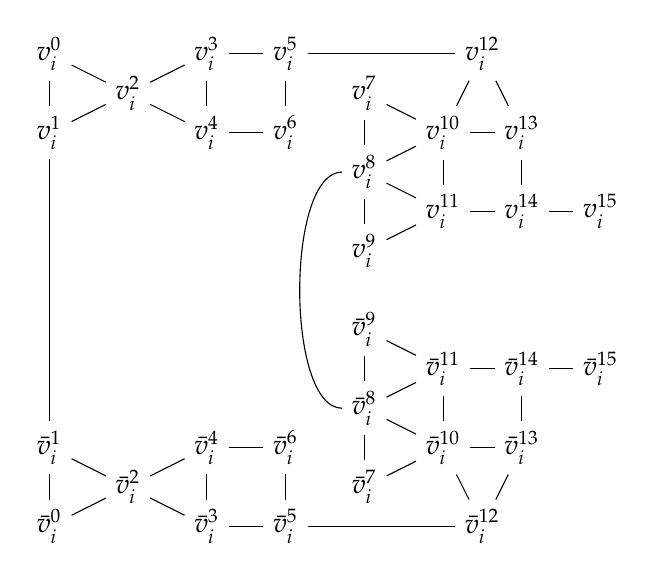
\begin{tikzpicture}
%\tikzstyle{place}=[circle,draw=blue!50,fill=blue!20,thick,inner sep=0pt,minimum size=6mm]
%\begin{scope}[every node/.style={circle,thick,draw,minimum size=3mm}]
\begin{scope}
    \node (A) at (0,3.5) {$v_i^0$};
    \node (B) at (0,2.5) {$v_i^1$};
    \node (C) at (1,3) {$v_i^2$};
    \node (D) at (2,3.5) {$v_i^3$};
    \node (E) at (2,2.5) {$v_i^4$};
    \node (F) at (3,3.5) {$v_i^5$};
    \node (G) at (3,2.5) {$v_i^6$};
    \node (H) at (4,3) {$v_i^7$};
    \node (I) at (4,2) {$v_i^8$};
    \node (J) at (4,1) {$v_i^9$};
    \node (K) at (5,2.5) {$v_i^{10}$};
    \node (L) at (5,1.5) {$v_i^{11}$};
    \node (M) at (5.5,3.5) {$v_i^{12}$};
    \node (N) at (6,2.5) {$v_i^{13}$};
    \node (O) at (6,1.5) {$v_i^{14}$};
    \node (P) at (7,1.5) {$v_i^{15}$};
    
    \node (a) at (0,-2.5) {$\bar{v}_i^0$};
    \node (b) at (0,-1.5) {$\bar{v}_i^1$};
    \node (c) at (1,-2) {$\bar{v}_i^2$};
    \node (d) at (2,-2.5) {$\bar{v}_i^3$};
    \node (e) at (2,-1.5) {$\bar{v}_i^4$};
    \node (f) at (3,-2.5) {$\bar{v}_i^5$};
    \node (g) at (3,-1.5) {$\bar{v}_i^6$};
    \node (h) at (4,-2) {$\bar{v}_i^7$};
    \node (i) at (4,-1) {$\bar{v}_i^8$};
    \node (j) at (4,0) {$\bar{v}_i^9$};
    \node (k) at (5,-1.5) {$\bar{v}_i^{10}$};
    \node (l) at (5,-0.5) {$\bar{v}_i^{11}$};
    \node (m) at (5.5,-2.5) {$\bar{v}_i^{12}$};
    \node (n) at (6,-1.5) {$\bar{v}_i^{13}$};
    \node (o) at (6,-0.5) {$\bar{v}_i^{14}$};
    \node (p) at (7,-0.5) {$\bar{v}_i^{15}$};
\end{scope}

\begin{scope}[>={Stealth[black]},
              every edge/.style={draw=black}]
    \path [-] (B) edge (b);
    \path [-] (A) edge (B);
    \path [-] (A) edge (C);
    \path [-] (B) edge (C);
    \path [-] (C) edge (D);
    \path [-] (C) edge (E);
    \path [-] (D) edge (E);
    \path [-] (D) edge (F);
    \path [-] (E) edge (G);
    \path [-] (F) edge (G);
    \path [-] (F) edge (M);
    \path [-] (H) edge (I);
    \path [-] (H) edge (K);
    \path [-] (K) edge (I);
    \path [-] (I) edge (J);
    \path [-] (I) edge (L);
    \path [-] (L) edge (J);
    \path [-] (K) edge (M);
    \path [-] (K) edge (N);
    \path [-] (K) edge (L);
    \path [-] (M) edge (N);
    \path [-] (N) edge (O);
    \path [-] (L) edge (O);
    \path [-] (O) edge (P);
    
    \path [-] (a) edge (b);
    \path [-] (a) edge (c);
    \path [-] (b) edge (c);
    \path [-] (c) edge (d);
    \path [-] (c) edge (e);
    \path [-] (d) edge (e);
    \path [-] (d) edge (f);
    \path [-] (e) edge (g);
    \path [-] (f) edge (g);
    \path [-] (f) edge (m);
    \path [-] (h) edge (i);
    \path [-] (h) edge (k);
    \path [-] (k) edge (i);
    \path [-] (i) edge (j);
    \path [-] (i) edge (l);
    \path [-] (l) edge (j);
    \path [-] (k) edge (m);
    \path [-] (k) edge (n);
    \path [-] (k) edge (l);
    \path [-] (m) edge (n);
    \path [-] (n) edge (o);
    \path [-] (l) edge (o);
    \path [-] (o) edge (p);
    
    %\path [-] (I) edge (i);
\end{scope}
\draw[-] (I) .. controls (3,2) and (3,-1) .. (i);
\end{tikzpicture}
\caption{A variable gadget that simulates the behaviour of a variable $v_i$. Each variable gadget consists of two symmetric parts, one for the variable (top) and one for its negation (bottom). The two parts are connected by the edge $v_i^8\bar{v}_i^8$, the direction of which decides whether the variable should be assigned \textit{TRUE} or \textit{FALSE} but not both to satisfy the 3-CNF problem.}
\label{fg:variable_gedget}
\end{figure}

% clause gadget
\begin{figure}[H]
\centering
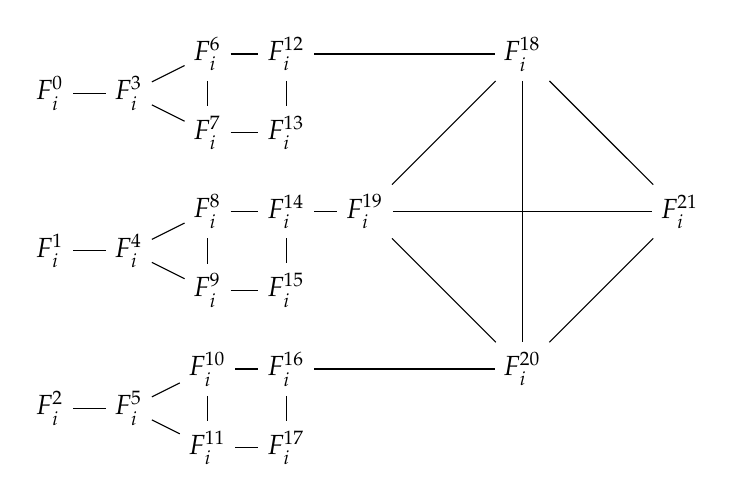
\begin{tikzpicture}
%\tikzstyle{place}=[circle,draw=blue!50,fill=blue!20,thick,inner sep=0pt,minimum size=6mm]
%\begin{scope}[every node/.style={circle,thick,draw,minimum size=3mm}]
\begin{scope}
    \node (a) at (0,4.5) {$F_i^0$};
    \node (b) at (0,2.5) {$F_i^1$};   
    \node (c) at (0,0.5) {$F_i^2$};
    \node (d) at (1,4.5) {$F_i^3$};
    \node (e) at (1,2.5) {$F_i^4$};
    \node (f) at (1,0.5) {$F_i^5$};
    \node (g) at (2,5) {$F_i^6$};
    \node (h) at (2,4) {$F_i^7$};
    \node (i) at (2,3) {$F_i^8$};
    \node (j) at (2,2) {$F_i^9$};
    \node (k) at (2,1) {$F_i^{10}$};
    \node (l) at (2,0) {$F_i^{11}$};
    \node (m) at (3,5) {$F_i^{12}$};
    \node (n) at (3,4) {$F_i^{13}$};
    \node (o) at (3,3) {$F_i^{14}$};
    \node (p) at (3,2) {$F_i^{15}$};
    \node (q) at (3,1) {$F_i^{16}$};
    \node (r) at (3,0) {$F_i^{17}$};
    \node (s) at (4,3) {$F_i^{19}$};
    \node (t) at (6,5) {$F_i^{18}$};
    \node (u) at (6,1) {$F_i^{20}$};
    \node (v) at (8,3) {$F_i^{21}$};
\end{scope}

\begin{scope}[>={Stealth[black]},every edge/.style={draw=black}]
    \path [-] (a) edge (d);
    \path [-] (d) edge (g);
    \path [-] (d) edge (h);
    \path [-] (g) edge (h);
    \path [-] (g) edge (m);
    \path [-] (h) edge (n);
    \path [-] (m) edge (n);
    \path [-] (m) edge (t);
    
    \path [-] (b) edge (e);
    \path [-] (i) edge (e);
    \path [-] (j) edge (e);
    \path [-] (i) edge (j);
    \path [-] (i) edge (o);
    \path [-] (j) edge (p);
    \path [-] (o) edge (p);
    \path [-] (o) edge (s);
    \path [-] (s) edge (u);
    \path [-] (s) edge (v);
    \path [-] (v) edge (u);
    \path [-] (t) edge (u);
    \path [-] (t) edge (v);
    \path [-] (t) edge (s);
    
    \path [-] (c) edge (f);
    \path [-] (f) edge (k);
    \path [-] (f) edge (l);
    \path [-] (k) edge (l);
    \path [-] (k) edge (q);
    \path [-] (l) edge (r);
    \path [-] (q) edge (r);
    \path [-] (q) edge (u);
\end{scope}
\end{tikzpicture}
\caption{A clause gadget that simulates the disjunction behaviour of a clause $F_i$. Each of the clause gadget consists of a $K_4$ and three envelope graphs, one for each variable that appears in the clause. The $K_4$ can be oriented into a DAG (with the same Markov blankets) s.t. any network flow comes into the $K_4$ only goes through one of the three envelope graphs, which connects to the \textit{TRUE} part of the corresponding variable gadget.}
\label{fg:clause_gedget}
\end{figure}

% auxiliary gadget
\begin{figure}[H]
\centering
\begin{tikzpicture}
\begin{scope}
    \node (a) at (1,4.5) {$S^0$};
    \node (b) at (2,5) {$S^1$};   
    \node (c) at (2,4) {$S^2$};
    \node (d) at (3,5) {$S^3$};
    \node (e) at (3,4) {$S^4$};
    
    \node (f) at (1,3) {$S^5$};
    \node (g) at (2,3) {$S^6$};
    \node (h) at (3,3) {$S^7_1$};
    \node (i) at (6,3) {$S^7_t$};
    
    \path [-] (a) edge (b);
    \path [-] (a) edge (c);
    \path [-] (b) edge (c);
    \path [-] (b) edge (d);
    \path [-] (c) edge (e);
    \path [-] (d) edge (e);
    \path [-] (f) edge (g);
	\path [-] (h) edge (g);
	\path [-] (h) edge (3.5,3);
	\path [-] (5.5,3) edge (i);
	\path [densely dashed] (4,3) edge (5,3);
\end{scope}
\end{tikzpicture}
\caption{The role of the auxiliary gadget is to connect the variable and clauses gadgets. It consists of an envelope graph, which is the smallest graph that can initialize a deterministic direction, and a chain of length $t+2$, in which node $S_i^7$ is connected to the clause gadget for $F_i$.}
\label{fg:aux_gedget}
\end{figure}

% partially directed 3-cnf
\begin{figure}[H]
\centering
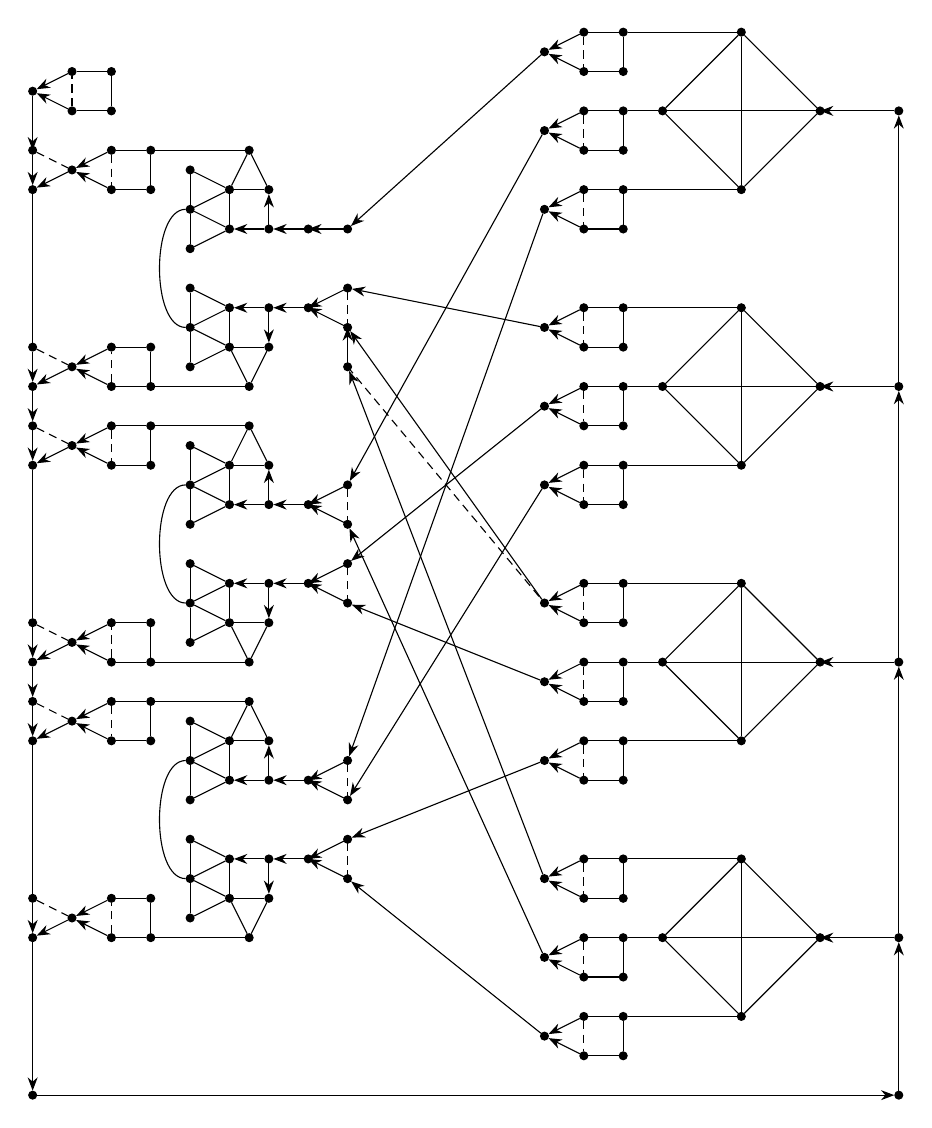
\begin{tikzpicture}
% variable gedget
\begin{scope}[every node/.style={circle,draw,fill=black,minimum size=1mm,inner sep=1pt},>={Stealth[black]}]
    \node (A) at (0,0.5) {};
    \node (B) at (0,1) {};
    \node (C) at (0.5,0.75) {};
    \node (D) at (1,0.5) {};
    \node (E) at (1,1) {};
    \node (F) at (1.5,0.5) {};
    \node (G) at (1.5,1) {};
    \node (H) at (2,0.75) {};
    \node (I) at (2,1.25) {};
    \node (J) at (2,1.75) {};
    \node (K) at (2.5,1) {};
    \node (L) at (2.5,1.5) {};
    \node (M) at (2.75,0.5) {};
    \node (N) at (3,1) {};
    \node (O) at (3,1.5) {};
    \node (P) at (3.5,1.5) {};
    \node (a) at (0,3.5) {};
    \node (b) at (0,3) {};
    \node (c) at (0.5,3.25) {};
    \node (d) at (1,3.5) {};
    \node (e) at (1,3) {};
    \node (f) at (1.5,3.5) {};
    \node (g) at (1.5,3) {};
    \node (h) at (2,3.25) {};
    \node (i) at (2,2.75) {};
    \node (j) at (2,2.25) {};
    \node (k) at (2.5,3) {};
    \node (l) at (2.5,2.5) {};
    \node (m) at (2.75,3.5) {};
    \node (n) at (3,3) {};
    \node (o) at (3,2.5) {};
    \node (p) at (3.5,2.5) {};
    
    \node (A1) at (0,0.5+3.5) {};
    \node (B1) at (0,1+3.5) {};
    \node (C1) at (0.5,0.75+3.5) {};
    \node (D1) at (1,0.5+3.5) {};
    \node (E1) at (1,1+3.5) {};
    \node (F1) at (1.5,0.5+3.5) {};
    \node (G1) at (1.5,1+3.5) {};
    \node (H1) at (2,0.75+3.5) {};
    \node (I1) at (2,1.25+3.5) {};
    \node (J1) at (2,1.75+3.5) {};
    \node (K1) at (2.5,1+3.5) {};
    \node (L1) at (2.5,1.5+3.5) {};
    \node (M1) at (2.75,0.5+3.5) {};
    \node (N1) at (3,1+3.5) {};
    \node (O1) at (3,1.5+3.5) {};
    \node (P1) at (3.5,1.5+3.5) {};
    \node (a1) at (0,3.5+3.5) {};
    \node (b1) at (0,3+3.5) {};
    \node (c1) at (0.5,3.25+3.5) {};
    \node (d1) at (1,3.5+3.5) {};
    \node (e1) at (1,3+3.5) {};
    \node (f1) at (1.5,3.5+3.5) {};
    \node (g1) at (1.5,3+3.5) {};
    \node (h1) at (2,3.25+3.5) {};
    \node (i1) at (2,2.75+3.5) {};
    \node (j1) at (2,2.25+3.5) {};
    \node (k1) at (2.5,3+3.5) {};
    \node (l1) at (2.5,2.5+3.5) {};
    \node (m1) at (2.75,3.5+3.5) {};
    \node (n1) at (3,3+3.5) {};
    \node (o1) at (3,2.5+3.5) {};
    \node (p1) at (3.5,2.5+3.5) {};
    
    \node (A2) at (0,0.5+7) {};
    \node (B2) at (0,1+7) {};
    \node (C2) at (0.5,0.75+7) {};
    \node (D2) at (1,0.5+7) {};
    \node (E2) at (1,1+7) {};
    \node (F2) at (1.5,0.5+7) {};
    \node (G2) at (1.5,1+7) {};
    \node (H2) at (2,0.75+7) {};
    \node (I2) at (2,1.25+7) {};
    \node (J2) at (2,1.75+7) {};
    \node (K2) at (2.5,1+7) {};
    \node (L2) at (2.5,1.5+7) {};
    \node (M2) at (2.75,0.5+7) {};
    \node (N2) at (3,1+7) {};
    \node (O2) at (3,1.5+7) {};
    \node (P2) at (3.5,1.5+7) {};
    \node (a2) at (0,3.5+7) {};
    \node (b2) at (0,3+7) {};
    \node (c2) at (0.5,3.25+7) {};
    \node (d2) at (1,3.5+7) {};
    \node (e2) at (1,3+7) {};
    \node (f2) at (1.5,3.5+7) {};
    \node (g2) at (1.5,3+7) {};
    \node (h2) at (2,3.25+7) {};
    \node (i2) at (2,2.75+7) {};
    \node (j2) at (2,2.25+7) {};
    \node (k2) at (2.5,3+7) {};
    \node (l2) at (2.5,2.5+7) {};
    \node (m2) at (2.75,3.5+7) {};
    \node (n2) at (3,3+7) {};
    \node (o2) at (3,2.5+7) {};
    \node (p2) at (3.5,2.5+7) {};

    \path [-] (B) edge (b);
    \path [->] (B) edge (A);
    \path [->] (C) edge (A);
    \path [densely dashed] (B) edge (C);
    \path [->] (D) edge (C);
    \path [->] (E) edge (C);
    \path [densely dashed] (D) edge (E);
    \path [-] (D) edge (F);
    \path [-] (E) edge (G);
    \path [-] (F) edge (G);
    \path [-] (F) edge (M);
    \path [-] (H) edge (I);
    \path [-] (H) edge (K);
    \path [-] (K) edge (I);
    \path [-] (I) edge (J);
    \path [-] (I) edge (L);
    \path [-] (L) edge (J);
    \path [-] (K) edge (M);
    \path [-] (K) edge (N);
    \path [-] (K) edge (L);
    \path [-] (M) edge (N);
    \path [->] (O) edge (N);
    \path [->] (O) edge (L);
    \path [->] (P) edge (O);
    \path [->] (a) edge (b);
    \path [densely dashed] (a) edge (c);
    \path [->] (c) edge (b);
    \path [->] (d) edge (c);
    \path [->] (e) edge (c);
    \path [densely dashed] (d) edge (e);
    \path [-] (d) edge (f);
    \path [-] (e) edge (g);
    \path [-] (f) edge (g);
    \path [-] (f) edge (m);
    \path [-] (h) edge (i);
    \path [-] (h) edge (k);
    \path [-] (k) edge (i);
    \path [-] (i) edge (j);
    \path [-] (i) edge (l);
    \path [-] (l) edge (j);
    \path [-] (k) edge (m);
    \path [-] (k) edge (n);
    \path [-] (k) edge (l);
    \path [-] (m) edge (n);
    \path [->] (o) edge (n);
    \path [->] (o) edge (l);
    \path [->] (p) edge (o);
    \draw[-] (I) .. controls (1.5,1.25) and (1.5,2.75) .. (i);
    
    \path [-] (B1) edge (b1);
    \path [->] (B1) edge (A1);
    \path [->] (C1) edge (A1);
    \path [densely dashed] (B1) edge (C1);
    \path [->] (D1) edge (C1);
    \path [->] (E1) edge (C1);
    \path [densely dashed] (D1) edge (E1);
    \path [-] (D1) edge (F1);
    \path [-] (E1) edge (G1);
    \path [-] (F1) edge (G1);
    \path [-] (F1) edge (M1);
    \path [-] (H1) edge (I1);
    \path [-] (H1) edge (K1);
    \path [-] (K1) edge (I1);
    \path [-] (I1) edge (J1);
    \path [-] (I1) edge (L1);
    \path [-] (L1) edge (J1);
    \path [-] (K1) edge (M1);
    \path [-] (K1) edge (N1);
    \path [-] (K1) edge (L1);
    \path [-] (M1) edge (N1);
    \path [->] (O1) edge (N1);
    \path [->] (O1) edge (L1);
    \path [->] (P1) edge (O1);
    \path [->] (a1) edge (b1);
    \path [densely dashed] (a1) edge (c1);
    \path [->] (c1) edge (b1);
    \path [->] (d1) edge (c1);
    \path [->] (e1) edge (c1);
    \path [densely dashed] (d1) edge (e1);
    \path [-] (d1) edge (f1);
    \path [-] (e1) edge (g1);
    \path [-] (f1) edge (g1);
    \path [-] (f1) edge (m1);
    \path [-] (h1) edge (i1);
    \path [-] (h1) edge (k1);
    \path [-] (k1) edge (i1);
    \path [-] (i1) edge (j1);
    \path [-] (i1) edge (l1);
    \path [-] (l1) edge (j1);
    \path [-] (k1) edge (m1);
    \path [-] (k1) edge (n1);
    \path [-] (k1) edge (l1);
    \path [-] (m1) edge (n1);
    \path [->] (o1) edge (n1);
    \path [->] (o1) edge (l1);
    \path [->] (p1) edge (o1);
    \draw[-] (I1) .. controls (1.5,1.25+3.5) and (1.5,2.75+3.5) .. (i1);
    
    \path [-] (B2) edge (b2);
    \path [->] (B2) edge (A2);
    \path [->] (C2) edge (A2);
    \path [densely dashed] (B2) edge (C2);
    \path [->] (D2) edge (C2);
    \path [->] (E2) edge (C2);
    \path [densely dashed] (D2) edge (E2);
    \path [-] (D2) edge (F2);
    \path [-] (E2) edge (G2);
    \path [-] (F2) edge (G2);
    \path [-] (F2) edge (M2);
    \path [-] (H2) edge (I2);
    \path [-] (H2) edge (K2);
    \path [-] (K2) edge (I2);
    \path [-] (I2) edge (J2);
    \path [-] (I2) edge (L2);
    \path [-] (L2) edge (J2);
    \path [-] (K2) edge (M2);
    \path [-] (K2) edge (N2);
    \path [-] (K2) edge (L2);
    \path [-] (M2) edge (N2);
    \path [->] (O2) edge (N2);
    \path [->] (O2) edge (L2);
    \path [->] (P2) edge (O2);
    \path [->] (a2) edge (b2);
    \path [densely dashed] (a2) edge (c2);
    \path [->] (c2) edge (b2);
    \path [->] (d2) edge (c2);
    \path [->] (e2) edge (c2);
    \path [densely dashed] (d2) edge (e2);
    \path [-] (d2) edge (f2);
    \path [-] (e2) edge (g2);
    \path [-] (f2) edge (g2);
    \path [-] (f2) edge (m2);
    \path [-] (h2) edge (i2);
    \path [-] (h2) edge (k2);
    \path [-] (k2) edge (i2);
    \path [-] (i2) edge (j2);
    \path [-] (i2) edge (l2);
    \path [-] (l2) edge (j2);
    \path [-] (k2) edge (m2);
    \path [-] (k2) edge (n2);
    \path [-] (k2) edge (l2);
    \path [-] (m2) edge (n2);
    \path [->] (o2) edge (n2);
    \path [->] (o2) edge (l2);
    \path [->] (p2) edge (o2);
    \draw[-] (I2) .. controls (1.5,1.25+7) and (1.5,2.75+7) .. (i2);
    
    \path [->] (A1) edge (a);
    \path [->] (A2) edge (a1);
\end{scope}

% clause gedget >={Stealth[black]},every node/.style={fill=white,circle},
\begin{scope}[every node/.style={circle,draw,fill=black,minimum size=1mm,inner sep=1pt},>={Stealth[black]}]
    \node (a) at (4,7.75) {};
    \path [->] (4,7.75) edge (4,8.25);
    \draw[densely dashed] (4,7.75) edge (6.5,4.75);
    \node (b) at (4,5.75) {};  
    \path [->] (4,5.75) edge (3.5,6); 
    \draw[densely dashed] (4,5.75) edge (4,6.25);
    \node (c) at (4,1.25) {};
    \path [->] (4,1.25) edge (3.5,1.5);
    \draw[densely dashed] (4,1.25) edge (4,1.75);
    \node (d) at (0+6.5,2.25-1) {};
    \node (e) at (0+6.5,1.25-1) {};
    \node (f) at (0+6.5,0.25-1) {};
    \node (g) at (0.5+6.5,2.5-1) {};
    \node (h) at (0.5+6.5,2-1) {};
    \node (i) at (0.5+6.5,1.5-1) {};
    \node (j) at (0.5+6.5,1-1) {};
    \node (k) at (0.5+6.5,0.5-1) {};
    \node (l) at (0.5+6.5,0-1) {};
    \node (m) at (1+6.5,2.5-1) {};
    \node (n) at (1+6.5,2-1) {};
    \node (o) at (1+6.5,1.5-1) {};
    \node (p) at (1+6.5,1-1) {};
    \node (q) at (1+6.5,0.5-1) {};
    \node (r) at (1+6.5,0-1) {};
    \node (s) at (1.5+6.5,1.5-1) {};
    \node (t) at (2.5+6.5,2.5-1) {};
    \node (u) at (2.5+6.5,0.5-1) {};
    \node (v) at (3.5+6.5,1.5-1) {};
    \path [<-] (a) edge (d);
    \path [<-] (d) edge (g);
    \path [<-] (d) edge (h);
    \path [densely dashed] (g) edge (h);
    \path [-] (g) edge (m);
    \path [-] (h) edge (n);
    \path [-] (m) edge (n);
    \path [-] (m) edge (t);
    \path [<-] (b) edge (e);
    \path [->] (i) edge (e);
    \path [->] (j) edge (e);
    \path [densely dashed] (i) edge (j);
    \path [-] (i) edge (o);
    \path [-] (j) edge (p);
    \path [-] (o) edge (p);
    \path [-] (o) edge (s);
    \path [-] (s) edge (u);
    \path [-] (s) edge (v);
    \path [-] (v) edge (u);
    \path [-] (t) edge (u);
    \path [-] (t) edge (v);
    \path [-] (t) edge (s);
    \path [<-] (c) edge (f);
    \path [<-] (f) edge (k);
    \path [<-] (f) edge (l);
    \path [densely dashed] (k) edge (l);
    \path [-] (k) edge (q);
    \path [-] (l) edge (r);
    \path [-] (q) edge (r);
    \path [-] (q) edge (u);
    
    \node (a1) at (4,8.25) {};
    \path [->] (4,8.25) edge (3.5,8.5);
    \draw[densely dashed] (4,8.25) edge (4,8.75);
    \node (b1) at (4,4.75) {};   
    \path [->] (4,4.75) edge (3.5,5);
    \draw[densely dashed] (4,4.75) edge (4,5.25);
    \node (c1) at (4,1.75) {};
    \path [->] (4,1.75) edge (3.5,1.5);
    \node (d1) at (0+6.5,2.25-1+3.5) {};
    \node (e1) at (0+6.5,1.25-1+3.5) {};
    \node (f1) at (0+6.5,0.25-1+3.5) {};
    \node (g1) at (0.5+6.5,2.5-1+3.5) {};
    \node (h1) at (0.5+6.5,2-1+3.5) {};
    \node (i1) at (0.5+6.5,1.5-1+3.5) {};
    \node (j1) at (0.5+6.5,1-1+3.5) {};
    \node (k1) at (0.5+6.5,0.5-1+3.5) {};
    \node (l1) at (0.5+6.5,0-1+3.5) {};
    \node (m1) at (1+6.5,2.5-1+3.5) {};
    \node (n1) at (1+6.5,2-1+3.5) {};
    \node (o1) at (1+6.5,1.5-1+3.5) {};
    \node (p1) at (1+6.5,1-1+3.5) {};
    \node (q1) at (1+6.5,0.5-1+3.5) {};
    \node (r1) at (1+6.5,0-1+3.5) {};
    \node (s1) at (1.5+6.5,1.5-1+3.5) {};
    \node (t1) at (2.5+6.5,2.5-1+3.5) {};
    \node (u1) at (2.5+6.5,0.5-1+3.5) {};
    \node (v1) at (3.5+6.5,1.5-1+3.5) {};
    \path [<-] (a1) edge (d1);
    \path [<-] (d1) edge (g1);
    \path [<-] (d1) edge (h1);
    \path [densely dashed] (g1) edge (h1);
    \path [-] (g1) edge (m1);
    \path [-] (h1) edge (n1);
    \path [-] (m1) edge (n1);
    \path [-] (m1) edge (t1);
    \path [<-] (b1) edge (e1);
    \path [->] (i1) edge (e1);
    \path [->] (j1) edge (e1);
    \path [densely dashed] (i1) edge (j1);
    \path [-] (i1) edge (o1);
    \path [-] (j1) edge (p1);
    \path [-] (o1) edge (p1);
    \path [-] (o1) edge (s1);
    \path [-] (s1) edge (u1);
    \path [-] (s1) edge (v1);
    \path [-] (v1) edge (u1);
    \path [-] (t1) edge (u1);
    \path [-] (t1) edge (v1);
    \path [-] (t1) edge (s1);
    \path [<-] (c1) edge (f1);
    \path [<-] (f1) edge (k1);
    \path [<-] (f1) edge (l1);
    \path [densely dashed] (k1) edge (l1);
    \path [-] (k1) edge (q1);
    \path [-] (l1) edge (r1);
    \path [-] (q1) edge (r1);
    \path [-] (q1) edge (u1);
    
    \node (a2) at (4,8.75) {};
    \path [->] (4,8.75) edge (3.5,8.5);
    \node (b2) at (4,5.25) {};   
    \path [->] (4,5.25) edge (3.5,5);
    \node (c2) at (4,2.25) {};
    \path [->] (4,2.25) edge (3.5,2.5);
    \draw[densely dashed] (4,2.25) edge (4,2.75);
    \node (d2) at (0+6.5,2.25-1+7) {};
    \node (e2) at (0+6.5,1.25-1+7) {};
    \node (f2) at (0+6.5,0.25-1+7) {};
    \node (g2) at (0.5+6.5,2.5-1+7) {};
    \node (h2) at (0.5+6.5,2-1+7) {};
    \node (i2) at (0.5+6.5,1.5-1+7) {};
    \node (j2) at (0.5+6.5,1-1+7) {};
    \node (k2) at (0.5+6.5,0.5-1+7) {};
    \node (l2) at (0.5+6.5,0-1+7) {};
    \node (m2) at (1+6.5,2.5-1+7) {};
    \node (n2) at (1+6.5,2-1+7) {};
    \node (o2) at (1+6.5,1.5-1+7) {};
    \node (p2) at (1+6.5,1-1+7) {};
    \node (q2) at (1+6.5,0.5-1+7) {};
    \node (r2) at (1+6.5,0-1+7) {};
    \node (s2) at (1.5+6.5,1.5-1+7) {};
    \node (t2) at (2.5+6.5,2.5-1+7) {};
    \node (u2) at (2.5+6.5,0.5-1+7) {};
    \node (v2) at (3.5+6.5,1.5-1+7) {};
    \path [<-] (a2) edge (d2);
    \path [<-] (d2) edge (g2);
    \path [<-] (d2) edge (h2);
    \path [densely dashed] (g2) edge (h2);
    \path [-] (g2) edge (m2);
    \path [-] (h2) edge (n2);
    \path [-] (m2) edge (n2);
    \path [-] (m2) edge (t2);
    \path [<-] (b2) edge (e2);
    \path [->] (i2) edge (e2);
    \path [->] (j2) edge (e2);
    \path [densely dashed] (i2) edge (j2);
    \path [-] (i2) edge (o2);
    \path [-] (j2) edge (p2);
    \path [-] (o2) edge (p2);
    \path [-] (o2) edge (s2);
    \path [-] (s2) edge (u2);
    \path [-] (s2) edge (v2);
    \path [-] (v2) edge (u2);
    \path [-] (t2) edge (u2);
    \path [-] (t2) edge (v2);
    \path [-] (t2) edge (s2);
    \path [<-] (c2) edge (f2);
    \path [<-] (f2) edge (k2);
    \path [<-] (f2) edge (l2);
    \path [densely dashed] (k2) edge (l2);
    \path [-] (k2) edge (q2);
    \path [-] (l2) edge (r2);
    \path [-] (q2) edge (r2);
    \path [-] (q2) edge (u2);
    
    \node (a4) at (4,9.5) {};
    \path [->] (4,9.5) edge (3.5,9.5);
    \node (b4) at (4,6.25) {};   
    \path [->] (4,6.25) edge (3.5,6);
    \node (c4) at (4,2.75) {};
    \path [->] (4,2.75) edge (3.5,2.5);
    \node (d4) at (0+6.5,2.25-1+10.5) {};
    \node (e4) at (0+6.5,1.25-1+10.5) {};
    \node (f4) at (0+6.5,0.25-1+10.5) {};
    \node (g4) at (0.5+6.5,2.5-1+10.5) {};
    \node (h4) at (0.5+6.5,2-1+10.5) {};
    \node (i4) at (0.5+6.5,1.5-1+10.5) {};
    \node (j4) at (0.5+6.5,1-1+10.5) {};
    \node (k4) at (0.5+6.5,0.5-1+10.5) {};
    \node (l4) at (0.5+6.5,0-1+10.5) {};
    \node (m4) at (1+6.5,2.5-1+10.5) {};
    \node (n4) at (1+6.5,2-1+10.5) {};
    \node (o4) at (1+6.5,1.5-1+10.5) {};
    \node (p4) at (1+6.5,1-1+10.5) {};
    \node (q4) at (1+6.5,0.5-1+10.5) {};
    \node (r4) at (1+6.5,0-1+10.5) {};
    \node (s4) at (1.5+6.5,1.5-1+10.5) {};
    \node (t4) at (2.5+6.5,2.5-1+10.5) {};
    \node (u4) at (2.5+6.5,0.5-1+10.5) {};
    \node (v4) at (3.5+6.5,1.5-1+10.5) {};
    \path [<-] (a4) edge (d4);
    \path [<-] (d4) edge (g4);
    \path [<-] (d4) edge (h4);
    \path [densely dashed] (g4) edge (h4);
    \path [-] (g4) edge (m4);
    \path [-] (h4) edge (n4);
    \path [-] (m4) edge (n4);
    \path [-] (m4) edge (t4);
    \path [<-] (b4) edge (e4);
    \path [->] (i4) edge (e4);
    \path [->] (j4) edge (e4);
    \path [densely dashed] (i4) edge (j4);
    \path [-] (i4) edge (o4);
    \path [-] (j4) edge (p4);
    \path [-] (o4) edge (p4);
    \path [-] (o4) edge (s4);
    \path [-] (s4) edge (u4);
    \path [-] (s4) edge (v4);
    \path [-] (v4) edge (u4);
    \path [-] (t4) edge (u4);
    \path [-] (t4) edge (v4);
    \path [-] (t4) edge (s4);
    \path [<-] (c4) edge (f4);
    \path [<-] (f4) edge (k4);
    \path [<-] (f4) edge (l4);
    \path [densely dashed] (k4) edge (l4);
    \path [-] (k4) edge (q4);
    \path [-] (l4) edge (r4);
    \path [-] (q4) edge (r4);
    \path [-] (q4) edge (u4);
\end{scope}

% auxiliary gedget
\begin{scope}[every node/.style={circle,draw,fill=black,minimum size=1mm,inner sep=1pt},>={Stealth[black]}]
    \node (a) at (0,11.25) {};
    \node (b) at (0.5,11.5) {};
    \node (c) at (0.5,11) {};
    \node (d) at (1,11.5) {};
    \node (e) at (1,11) {};
    \path [<-] (a) edge (b);
    \path [<-] (a) edge (c);
    \path [densely dashed] (c) edge (b);
    \path [-] (d) edge (b);
    \path [-] (c) edge (e);
    \path [-] (d) edge (e);
    \path [->] (a) edge (0,10.5);
    
    \node (f) at (0,-1.5) {};
    \path[->] (0,0.5) edge (f);
    
    \node (g) at (11,-1.5) {};
    \node (h) at (11,0.5) {};
    \node (i) at (11,4) {};
    \node (j) at (11,7.5) {};
    \node (k) at (11,11) {};                
    \path [->] (f) edge (g);
    \path [->] (g) edge (h);
    \path [->] (h) edge (i);
    \path [->] (i) edge (j);
    \path [->] (j) edge (k);
    \path [->] (h) edge (10,0.5);
    \path [->] (i) edge (10,4);
    \path [->] (j) edge (10,7.5);
    \path [->] (k) edge (10,11);
\end{scope}
\end{tikzpicture}
\caption{A polynomial time reduction from a 3-CNF problem to a graph morality problem. The 3-CNF logic formula is $(X \vee Y \vee Z)\wedge(\bar{X} \vee \bar{Y} \vee Z)\wedge(\bar{X} \vee \bar{Y} \vee \bar{Z})\wedge(\bar{X} \vee Y \vee \bar{Z})$. From top to bottom in the graph, the variable gadgets are for variables $X, Y, Z$ and the clause gadgets are for clauses $F_1,F_2,F_3,F_4$. This construction guarantees the resulting graph has maximum degree $5$. The directed and deleted edges in the graph are determined by envelope graphs, and they stay unchanged under any conditions.}
\label{fg:3cnf_partial_dir}
\end{figure}


% fully directed 3-cnf 
\begin{figure}[H]
\centering
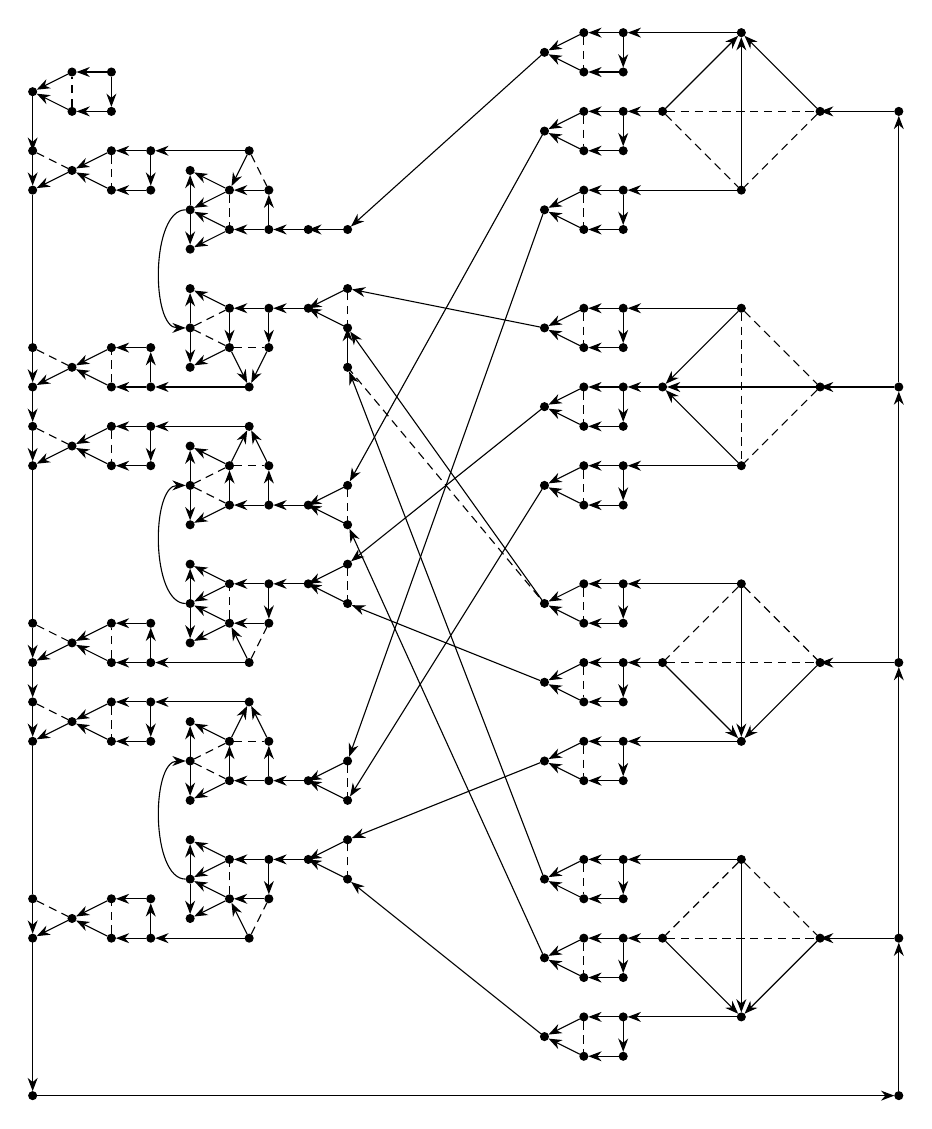
\begin{tikzpicture}
% variable gedget
\begin{scope}[every node/.style={circle,draw,fill=black,minimum size=1mm,inner sep=1pt},>={Stealth[black]}]
    \node (A) at (0,0.5) {};
    \node (B) at (0,1) {};
    \node (C) at (0.5,0.75) {};
    \node (D) at (1,0.5) {};
    \node (E) at (1,1) {};
    \node (F) at (1.5,0.5) {};
    \node (G) at (1.5,1) {};
    \node (H) at (2,0.75) {};
    \node (I) at (2,1.25) {};
    \node (J) at (2,1.75) {};
    \node (K) at (2.5,1) {};
    \node (L) at (2.5,1.5) {};
    \node (M) at (2.75,0.5) {};
    \node (N) at (3,1) {};
    \node (O) at (3,1.5) {};
    \node (P) at (3.5,1.5) {};
    \node (a) at (0,3.5) {};
    \node (b) at (0,3) {};
    \node (c) at (0.5,3.25) {};
    \node (d) at (1,3.5) {};
    \node (e) at (1,3) {};
    \node (f) at (1.5,3.5) {};
    \node (g) at (1.5,3) {};
    \node (h) at (2,3.25) {};
    \node (i) at (2,2.75) {};
    \node (j) at (2,2.25) {};
    \node (k) at (2.5,3) {};
    \node (l) at (2.5,2.5) {};
    \node (m) at (2.75,3.5) {};
    \node (n) at (3,3) {};
    \node (o) at (3,2.5) {};
    \node (p) at (3.5,2.5) {};
    
    \node (A1) at (0,0.5+3.5) {};
    \node (B1) at (0,1+3.5) {};
    \node (C1) at (0.5,0.75+3.5) {};
    \node (D1) at (1,0.5+3.5) {};
    \node (E1) at (1,1+3.5) {};
    \node (F1) at (1.5,0.5+3.5) {};
    \node (G1) at (1.5,1+3.5) {};
    \node (H1) at (2,0.75+3.5) {};
    \node (I1) at (2,1.25+3.5) {};
    \node (J1) at (2,1.75+3.5) {};
    \node (K1) at (2.5,1+3.5) {};
    \node (L1) at (2.5,1.5+3.5) {};
    \node (M1) at (2.75,0.5+3.5) {};
    \node (N1) at (3,1+3.5) {};
    \node (O1) at (3,1.5+3.5) {};
    \node (P1) at (3.5,1.5+3.5) {};
    \node (a1) at (0,3.5+3.5) {};
    \node (b1) at (0,3+3.5) {};
    \node (c1) at (0.5,3.25+3.5) {};
    \node (d1) at (1,3.5+3.5) {};
    \node (e1) at (1,3+3.5) {};
    \node (f1) at (1.5,3.5+3.5) {};
    \node (g1) at (1.5,3+3.5) {};
    \node (h1) at (2,3.25+3.5) {};
    \node (i1) at (2,2.75+3.5) {};
    \node (j1) at (2,2.25+3.5) {};
    \node (k1) at (2.5,3+3.5) {};
    \node (l1) at (2.5,2.5+3.5) {};
    \node (m1) at (2.75,3.5+3.5) {};
    \node (n1) at (3,3+3.5) {};
    \node (o1) at (3,2.5+3.5) {};
    \node (p1) at (3.5,2.5+3.5) {};
    
    \node (A2) at (0,0.5+7) {};
    \node (B2) at (0,1+7) {};
    \node (C2) at (0.5,0.75+7) {};
    \node (D2) at (1,0.5+7) {};
    \node (E2) at (1,1+7) {};
    \node (F2) at (1.5,0.5+7) {};
    \node (G2) at (1.5,1+7) {};
    \node (H2) at (2,0.75+7) {};
    \node (I2) at (2,1.25+7) {};
    \node (J2) at (2,1.75+7) {};
    \node (K2) at (2.5,1+7) {};
    \node (L2) at (2.5,1.5+7) {};
    \node (M2) at (2.75,0.5+7) {};
    \node (N2) at (3,1+7) {};
    \node (O2) at (3,1.5+7) {};
    \node (P2) at (3.5,1.5+7) {};
    \node (a2) at (0,3.5+7) {};
    \node (b2) at (0,3+7) {};
    \node (c2) at (0.5,3.25+7) {};
    \node (d2) at (1,3.5+7) {};
    \node (e2) at (1,3+7) {};
    \node (f2) at (1.5,3.5+7) {};
    \node (g2) at (1.5,3+7) {};
    \node (h2) at (2,3.25+7) {};
    \node (i2) at (2,2.75+7) {};
    \node (j2) at (2,2.25+7) {};
    \node (k2) at (2.5,3+7) {};
    \node (l2) at (2.5,2.5+7) {};
    \node (m2) at (2.75,3.5+7) {};
    \node (n2) at (3,3+7) {};
    \node (o2) at (3,2.5+7) {};
    \node (p2) at (3.5,2.5+7) {};
    % Z
    \path [-] (B) edge (b);
    \path [->] (B) edge (A);
    \path [->] (C) edge (A);
    \path [densely dashed] (B) edge (C);
    \path [->] (D) edge (C);
    \path [->] (E) edge (C);
    \path [densely dashed] (D) edge (E);
    \path [<-] (D) edge (F);
    \path [<-] (E) edge (G);
    \path [->] (F) edge (G);
    \path [<-] (F) edge (M);
    \path [<-] (H) edge (I);
    \path [<-] (H) edge (K);
    \path [->] (K) edge (I);
    \path [->] (I) edge (J);
    \path [<-] (I) edge (L);
    \path [->] (L) edge (J);
    \path [<-] (K) edge (M);
    \path [<-] (K) edge (N);
    \path [densely dashed] (K) edge (L);
    \path [densely dashed] (M) edge (N);
    \path [->] (O) edge (N);
    \path [->] (O) edge (L);
    \path [->] (P) edge (O);
    \path [->] (a) edge (b);
    \path [densely dashed] (a) edge (c);
    \path [->] (c) edge (b);
    \path [->] (d) edge (c);
    \path [->] (e) edge (c);
    \path [densely dashed] (d) edge (e);
   \path [<-] (d) edge (f);
    \path [<-] (e) edge (g);
    \path [->] (f) edge (g);
    \path [<-] (f) edge (m);
    \path [<-] (h) edge (i);
    \path [<-] (h) edge (k);
    \path [densely dashed] (k) edge (i);
    \path [->] (i) edge (j);
    \path [densely dashed] (i) edge (l);
    \path [->] (l) edge (j);
    \path [->] (k) edge (m);
    \path [densely dashed] (k) edge (n);
    \path [<-] (k) edge (l);
    \path [<-] (m) edge (n);
    \path [->] (o) edge (n);
    \path [->] (o) edge (l);
    \path [->] (p) edge (o);
    \draw[->] (I) .. controls (1.5,1.25) and (1.5,2.75) .. (i);
    % Y
    \path [-] (B1) edge (b1);
    \path [->] (B1) edge (A1);
    \path [->] (C1) edge (A1);
    \path [densely dashed] (B1) edge (C1);
    \path [->] (D1) edge (C1);
    \path [->] (E1) edge (C1);
    \path [densely dashed] (D1) edge (E1);
    \path [<-] (d1) edge (f1);
    \path [<-] (e1) edge (g1);
    \path [->] (f1) edge (g1);
    \path [<-] (f1) edge (m1);
    \path [<-] (h1) edge (i1);
    \path [<-] (h1) edge (k1);
    \path [densely dashed] (k1) edge (i1);
    \path [->] (i1) edge (j1);
    \path [densely dashed] (i1) edge (l1);
    \path [->] (l1) edge (j1);
    \path [->] (k1) edge (m1);
    \path [densely dashed] (k1) edge (n1);
    \path [<-] (k1) edge (l1);
    \path [<-] (m1) edge (n1);
    \path [->] (O1) edge (N1);
    \path [->] (O1) edge (L1);
    \path [->] (P1) edge (O1);
    \path [->] (a1) edge (b1);
    \path [densely dashed] (a1) edge (c1);
    \path [->] (c1) edge (b1);
    \path [->] (d1) edge (c1);
    \path [->] (e1) edge (c1);
    \path [densely dashed] (d1) edge (e1);
    \path [<-] (D1) edge (F1);
    \path [<-] (E1) edge (G1);
    \path [->] (F1) edge (G1);
    \path [<-] (F1) edge (M1);
    \path [<-] (H1) edge (I1);
    \path [<-] (H1) edge (K1);
    \path [->] (K1) edge (I1);
    \path [->] (I1) edge (J1);
    \path [<-] (I1) edge (L1);
    \path [->] (L1) edge (J1);
    \path [<-] (K1) edge (M1);
    \path [<-] (K1) edge (N1);
    \path [densely dashed] (K1) edge (L1);
    \path [densely dashed] (M1) edge (N1);
    \path [->] (o1) edge (n1);
    \path [->] (o1) edge (l1);
    \path [->] (p1) edge (o1);
    \draw[->] (I1) .. controls (1.5,1.25+3.5) and (1.5,2.75+3.5) .. (i1);
    % X
    \path [-] (B2) edge (b2);
    \path [->] (B2) edge (A2);
    \path [->] (C2) edge (A2);
    \path [densely dashed] (B2) edge (C2);
    \path [->] (D2) edge (C2);
    \path [->] (E2) edge (C2);
    \path [densely dashed] (D2) edge (E2);
    \path [<-] (D2) edge (F2);
    \path [<-] (E2) edge (G2);
    \path [->] (F2) edge (G2);
    \path [<-] (F2) edge (M2);
    \path [<-] (H2) edge (I2);
    \path [<-] (H2) edge (K2);
    \path [densely dashed] (K2) edge (I2);
    \path [->] (I2) edge (J2);
    \path [densely dashed] (I2) edge (L2);
    \path [->] (L2) edge (J2);
    \path [->] (K2) edge (M2);
    \path [densely dashed] (K2) edge (N2);
    \path [<-] (K2) edge (L2);
    \path [<-] (M2) edge (N2);
    \path [->] (O2) edge (N2);
    \path [->] (O2) edge (L2);
    \path [->] (P2) edge (O2);
    \path [->] (a2) edge (b2);
    \path [densely dashed] (a2) edge (c2);
    \path [->] (c2) edge (b2);
    \path [->] (d2) edge (c2);
    \path [->] (e2) edge (c2);
    \path [densely dashed] (d2) edge (e2);
    \path [<-] (d2) edge (f2);
    \path [<-] (e2) edge (g2);
    \path [->] (f2) edge (g2);
    \path [<-] (f2) edge (m2);
    \path [<-] (h2) edge (i2);
    \path [<-] (h2) edge (k2);
    \path [->] (k2) edge (i2);
    \path [->] (i2) edge (j2);
    \path [<-] (i2) edge (l2);
    \path [->] (l2) edge (j2);
    \path [<-] (k2) edge (m2);
    \path [<-] (k2) edge (n2);
    \path [densely dashed] (k2) edge (l2);
    \path [densely dashed] (m2) edge (n2);
    \path [->] (o2) edge (n2);
    \path [->] (o2) edge (l2);
    \path [->] (p2) edge (o2);
    \draw[<-] (I2) .. controls (1.5,1.25+7) and (1.5,2.75+7) .. (i2);
    
    \path [->] (A1) edge (a);
    \path [->] (A2) edge (a1);
\end{scope}

% clause gedget >={Stealth[black]},every node/.style={fill=white,circle},
\begin{scope}[every node/.style={circle,draw,fill=black,minimum size=1mm,inner sep=1pt},>={Stealth[black]}]
    % F4
    \node (a) at (4,7.75) {};
    \path [->] (4,7.75) edge (4,8.25);
    \draw[densely dashed] (4,7.75) edge (6.5,4.75);
    \node (b) at (4,5.75) {};  
    \path [->] (4,5.75) edge (3.5,6); 
    \draw[densely dashed] (4,5.75) edge (4,6.25);
    \node (c) at (4,1.25) {};
    \path [->] (4,1.25) edge (3.5,1.5);
    \draw[densely dashed] (4,1.25) edge (4,1.75);
    \node (d) at (0+6.5,2.25-1) {};
    \node (e) at (0+6.5,1.25-1) {};
    \node (f) at (0+6.5,0.25-1) {};
    \node (g) at (0.5+6.5,2.5-1) {};
    \node (h) at (0.5+6.5,2-1) {};
    \node (i) at (0.5+6.5,1.5-1) {};
    \node (j) at (0.5+6.5,1-1) {};
    \node (k) at (0.5+6.5,0.5-1) {};
    \node (l) at (0.5+6.5,0-1) {};
    \node (m) at (1+6.5,2.5-1) {};
    \node (n) at (1+6.5,2-1) {};
    \node (o) at (1+6.5,1.5-1) {};
    \node (p) at (1+6.5,1-1) {};
    \node (q) at (1+6.5,0.5-1) {};
    \node (r) at (1+6.5,0-1) {};
    \node (s) at (1.5+6.5,1.5-1) {};
    \node (t) at (2.5+6.5,2.5-1) {};
    \node (u) at (2.5+6.5,0.5-1) {};
    \node (v) at (3.5+6.5,1.5-1) {};
    \path [<-] (a) edge (d);
    \path [<-] (d) edge (g);
    \path [<-] (d) edge (h);
    \path [densely dashed] (g) edge (h);
    \path [<-] (g) edge (m);
    \path [<-] (h) edge (n);
    \path [->] (m) edge (n);
    \path [<-] (m) edge (t);
    \path [<-] (b) edge (e);
    \path [->] (i) edge (e);
    \path [->] (j) edge (e);
    \path [densely dashed] (i) edge (j);
    \path [<-] (i) edge (o);
    \path [<-] (j) edge (p);
    \path [->] (o) edge (p);
    \path [<-] (o) edge (s);
    \path [->] (s) edge (u);
    \path [densely dashed] (s) edge (v);
    \path [->] (v) edge (u);
    \path [->] (t) edge (u);
    \path [densely dashed] (t) edge (v);
    \path [densely dashed] (t) edge (s);
    \path [<-] (c) edge (f);
    \path [<-] (f) edge (k);
    \path [<-] (f) edge (l);
    \path [densely dashed] (k) edge (l);
    \path [<-] (k) edge (q);
    \path [<-] (l) edge (r);
    \path [->] (q) edge (r);
    \path [<-] (q) edge (u);
    % F3
    \node (a1) at (4,8.25) {};
    \path [->] (4,8.25) edge (3.5,8.5);
    \draw[densely dashed] (4,8.25) edge (4,8.75);
    \node (b1) at (4,4.75) {};   
    \path [->] (4,4.75) edge (3.5,5);
    \draw[densely dashed] (4,4.75) edge (4,5.25);
    \node (c1) at (4,1.75) {};
    \path [->] (4,1.75) edge (3.5,1.5);
    \node (d1) at (0+6.5,2.25-1+3.5) {};
    \node (e1) at (0+6.5,1.25-1+3.5) {};
    \node (f1) at (0+6.5,0.25-1+3.5) {};
    \node (g1) at (0.5+6.5,2.5-1+3.5) {};
    \node (h1) at (0.5+6.5,2-1+3.5) {};
    \node (i1) at (0.5+6.5,1.5-1+3.5) {};
    \node (j1) at (0.5+6.5,1-1+3.5) {};
    \node (k1) at (0.5+6.5,0.5-1+3.5) {};
    \node (l1) at (0.5+6.5,0-1+3.5) {};
    \node (m1) at (1+6.5,2.5-1+3.5) {};
    \node (n1) at (1+6.5,2-1+3.5) {};
    \node (o1) at (1+6.5,1.5-1+3.5) {};
    \node (p1) at (1+6.5,1-1+3.5) {};
    \node (q1) at (1+6.5,0.5-1+3.5) {};
    \node (r1) at (1+6.5,0-1+3.5) {};
    \node (s1) at (1.5+6.5,1.5-1+3.5) {};
    \node (t1) at (2.5+6.5,2.5-1+3.5) {};
    \node (u1) at (2.5+6.5,0.5-1+3.5) {};
    \node (v1) at (3.5+6.5,1.5-1+3.5) {};
    \path [<-] (a1) edge (d1);
    \path [<-] (d1) edge (g1);
    \path [<-] (d1) edge (h1);
    \path [densely dashed] (g1) edge (h1);
    \path [<-] (g1) edge (m1);
    \path [<-] (h1) edge (n1);
    \path [->] (m1) edge (n1);
    \path [<-] (m1) edge (t1);
    \path [<-] (b1) edge (e1);
    \path [->] (i1) edge (e1);
    \path [->] (j1) edge (e1);
    \path [densely dashed] (i1) edge (j1);
    \path [<-] (i1) edge (o1);
    \path [<-] (j1) edge (p1);
    \path [->] (o1) edge (p1);
    \path [<-] (o1) edge (s1);
    \path [->] (s1) edge (u1);
    \path [densely dashed] (s1) edge (v1);
    \path [->] (v1) edge (u1);
    \path [->] (t1) edge (u1);
    \path [densely dashed] (t1) edge (v1);
    \path [densely dashed] (t1) edge (s1);
    \path [<-] (c1) edge (f1);
    \path [<-] (f1) edge (k1);
    \path [<-] (f1) edge (l1);
    \path [densely dashed] (k1) edge (l1);
    \path [<-] (k1) edge (q1);
    \path [<-] (l1) edge (r1);
    \path [->] (q1) edge (r1);
    \path [<-] (q1) edge (u1);
    % F2
    \node (a2) at (4,8.75) {};
    \path [->] (4,8.75) edge (3.5,8.5);
    \node (b2) at (4,5.25) {};   
    \path [->] (4,5.25) edge (3.5,5);
    \node (c2) at (4,2.25) {};
    \path [->] (4,2.25) edge (3.5,2.5);
    \draw[densely dashed] (4,2.25) edge (4,2.75);
    \node (d2) at (0+6.5,2.25-1+7) {};
    \node (e2) at (0+6.5,1.25-1+7) {};
    \node (f2) at (0+6.5,0.25-1+7) {};
    \node (g2) at (0.5+6.5,2.5-1+7) {};
    \node (h2) at (0.5+6.5,2-1+7) {};
    \node (i2) at (0.5+6.5,1.5-1+7) {};
    \node (j2) at (0.5+6.5,1-1+7) {};
    \node (k2) at (0.5+6.5,0.5-1+7) {};
    \node (l2) at (0.5+6.5,0-1+7) {};
    \node (m2) at (1+6.5,2.5-1+7) {};
    \node (n2) at (1+6.5,2-1+7) {};
    \node (o2) at (1+6.5,1.5-1+7) {};
    \node (p2) at (1+6.5,1-1+7) {};
    \node (q2) at (1+6.5,0.5-1+7) {};
    \node (r2) at (1+6.5,0-1+7) {};
    \node (s2) at (1.5+6.5,1.5-1+7) {};
    \node (t2) at (2.5+6.5,2.5-1+7) {};
    \node (u2) at (2.5+6.5,0.5-1+7) {};
    \node (v2) at (3.5+6.5,1.5-1+7) {};
    \path [<-] (a2) edge (d2);
    \path [<-] (d2) edge (g2);
    \path [<-] (d2) edge (h2);
    \path [densely dashed] (g2) edge (h2);
    \path [<-] (g2) edge (m2);
    \path [<-] (h2) edge (n2);
    \path [->] (m2) edge (n2);
    \path [<-] (m2) edge (t2);
    \path [<-] (b2) edge (e2);
    \path [->] (i2) edge (e2);
    \path [->] (j2) edge (e2);
    \path [densely dashed] (i2) edge (j2);
    \path [<-] (i2) edge (o2);
    \path [<-] (j2) edge (p2);
    \path [->] (o2) edge (p2);
    \path [<-] (o2) edge (s2);
    \path [<-] (s2) edge (u2);
    \path [<-] (s2) edge (v2);
    \path [densely dashed] (v2) edge (u2);
    \path [densely dashed] (t2) edge (u2);
    \path [densely dashed] (t2) edge (v2);
    \path [->] (t2) edge (s2);
    \path [<-] (c2) edge (f2);
    \path [<-] (f2) edge (k2);
    \path [<-] (f2) edge (l2);
    \path [densely dashed] (k2) edge (l2);
    \path [<-] (k2) edge (q2);
    \path [<-] (l2) edge (r2);
    \path [->] (q2) edge (r2);
    \path [<-] (q2) edge (u2);
    % F1
    \node (a4) at (4,9.5) {};
    \path [->] (4,9.5) edge (3.5,9.5);
    \node (b4) at (4,6.25) {};   
    \path [->] (4,6.25) edge (3.5,6);
    \node (c4) at (4,2.75) {};
    \path [->] (4,2.75) edge (3.5,2.5);
    \node (d4) at (0+6.5,2.25-1+10.5) {};
    \node (e4) at (0+6.5,1.25-1+10.5) {};
    \node (f4) at (0+6.5,0.25-1+10.5) {};
    \node (g4) at (0.5+6.5,2.5-1+10.5) {};
    \node (h4) at (0.5+6.5,2-1+10.5) {};
    \node (i4) at (0.5+6.5,1.5-1+10.5) {};
    \node (j4) at (0.5+6.5,1-1+10.5) {};
    \node (k4) at (0.5+6.5,0.5-1+10.5) {};
    \node (l4) at (0.5+6.5,0-1+10.5) {};
    \node (m4) at (1+6.5,2.5-1+10.5) {};
    \node (n4) at (1+6.5,2-1+10.5) {};
    \node (o4) at (1+6.5,1.5-1+10.5) {};
    \node (p4) at (1+6.5,1-1+10.5) {};
    \node (q4) at (1+6.5,0.5-1+10.5) {};
    \node (r4) at (1+6.5,0-1+10.5) {};
    \node (s4) at (1.5+6.5,1.5-1+10.5) {};
    \node (t4) at (2.5+6.5,2.5-1+10.5) {};
    \node (u4) at (2.5+6.5,0.5-1+10.5) {};
    \node (v4) at (3.5+6.5,1.5-1+10.5) {};
    \path [<-] (a4) edge (d4);
    \path [<-] (d4) edge (g4);
    \path [<-] (d4) edge (h4);
    \path [densely dashed] (g4) edge (h4);
    \path [<-] (g4) edge (m4);
    \path [<-] (h4) edge (n4);
    \path [->] (m4) edge (n4);
    \path [<-] (m4) edge (t4);
    \path [<-] (b4) edge (e4);
    \path [->] (i4) edge (e4);
    \path [->] (j4) edge (e4);
    \path [densely dashed] (i4) edge (j4);
    \path [<-] (i4) edge (o4);
    \path [<-] (j4) edge (p4);
    \path [->] (o4) edge (p4);
    \path [<-] (o4) edge (s4);
    \path [densely dashed] (s4) edge (u4);
    \path [densely dashed] (s4) edge (v4);
    \path [densely dashed] (v4) edge (u4);
    \path [<-] (t4) edge (u4);
    \path [<-] (t4) edge (v4);
    \path [<-] (t4) edge (s4);
    \path [<-] (c4) edge (f4);
    \path [<-] (f4) edge (k4);
    \path [<-] (f4) edge (l4);
    \path [densely dashed] (k4) edge (l4);
    \path [<-] (k4) edge (q4);
    \path [<-] (l4) edge (r4);
    \path [->] (q4) edge (r4);
    \path [<-] (q4) edge (u4);
\end{scope}

% auxiliary gedget
\begin{scope}[every node/.style={circle,draw,fill=black,minimum size=1mm,inner sep=1pt},>={Stealth[black]}]
    \node (a) at (0,11.25) {};
    \node (b) at (0.5,11.5) {};
    \node (c) at (0.5,11) {};
    \node (d) at (1,11.5) {};
    \node (e) at (1,11) {};
    \path [<-] (a) edge (b);
    \path [<-] (a) edge (c);
    \path [densely dashed] (c) edge (b);
    \path [->] (d) edge (b);
    \path [<-] (c) edge (e);
    \path [->] (d) edge (e);
    \path [->] (a) edge (0,10.5);
    
    \node (f) at (0,-1.5) {};
    \path[->] (0,0.5) edge (f);
    
    \node (g) at (11,-1.5) {};
    \node (h) at (11,0.5) {};
    \node (i) at (11,4) {};
    \node (j) at (11,7.5) {};
    \node (k) at (11,11) {};                
    \path [->] (f) edge (g);
    \path [->] (g) edge (h);
    \path [->] (h) edge (i);
    \path [->] (i) edge (j);
    \path [->] (j) edge (k);
    \path [->] (h) edge (10,0.5);
    \path [->] (i) edge (10,4);
    \path [->] (j) edge (10,7.5);
    \path [->] (k) edge (10,11);
\end{scope}
\end{tikzpicture}
\caption{A polynomial time reduction from a 3-CNF problem to a graph morality problem. The 3-CNF problem is $(X \vee Y \vee Z)\wedge(\bar{X} \vee \bar{Y} \vee Z)\wedge(\bar{X} \vee \bar{Y} \vee \bar{Z})\wedge(\bar{X} \vee Y \vee \bar{Z})$, where $X=1$ and $Y=Z=0$. From top to bottom, the variable gadgets are $X, Y, Z$ and the clause gadgets are $F_1,F_2,F_3,F_4$. This construction guarantees the resulting graph has maximum degree $5$.}
\label{fg:3cnf_fully_dir}
\end{figure}


\bibliographystyle{named}
\bibliography{causal_discovery_ref_list}

\end{document}